\documentclass[11pt]{book}

\usepackage[top=1.25in,bottom=1.25in,right=1in,left=1in]{geometry}
\usepackage[colorlinks=true, urlcolor=blue, linkcolor=violet ]{hyperref}
\usepackage{graphicx}
\usepackage{caption}
\usepackage{listings}
\usepackage{pgfplots}
\usetikzlibrary{calc,angles,quotes}
\usepackage{tikz}
\usepackage{booktabs}
\usepackage[titletoc]{appendix} 
\usepackage{xepersian}
\usepackage{lmodern} 
\usepackage{amsmath}
\usepackage{amssymb}
\usepackage{fancyhdr}

\lstset{basicstyle=\ttfamily\small}

\settextfont[Scale=1.1]{XB Niloofar}
\setlatintextfont[Scale=1.0]{Times New Roman}
\setdigitfont[Scale=1.1]{XB Niloofar}

\newcommand{\len}[1]{\lr{#1}}

\title{پاسخنامه الکترومغناطیس ریتس و میلفورد + تحلیل محاسباتی}
\author{S.Mustafa}
\date{}

\counterwithin{equation}{section}
\counterwithin{figure}{section}
\counterwithin{footnote}{section}

\begin{document}

\maketitle
\newpage

\tableofcontents

\newpage

\section{فصل اول: آنالیز برداری}

\section{فصل دوم: الکترواستاتیک}

\subsection{}
\begin{figure}[h!]
  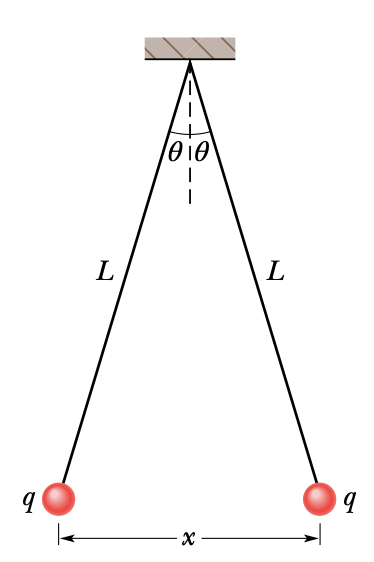
\includegraphics[width=0.4\textwidth]{2.1}
  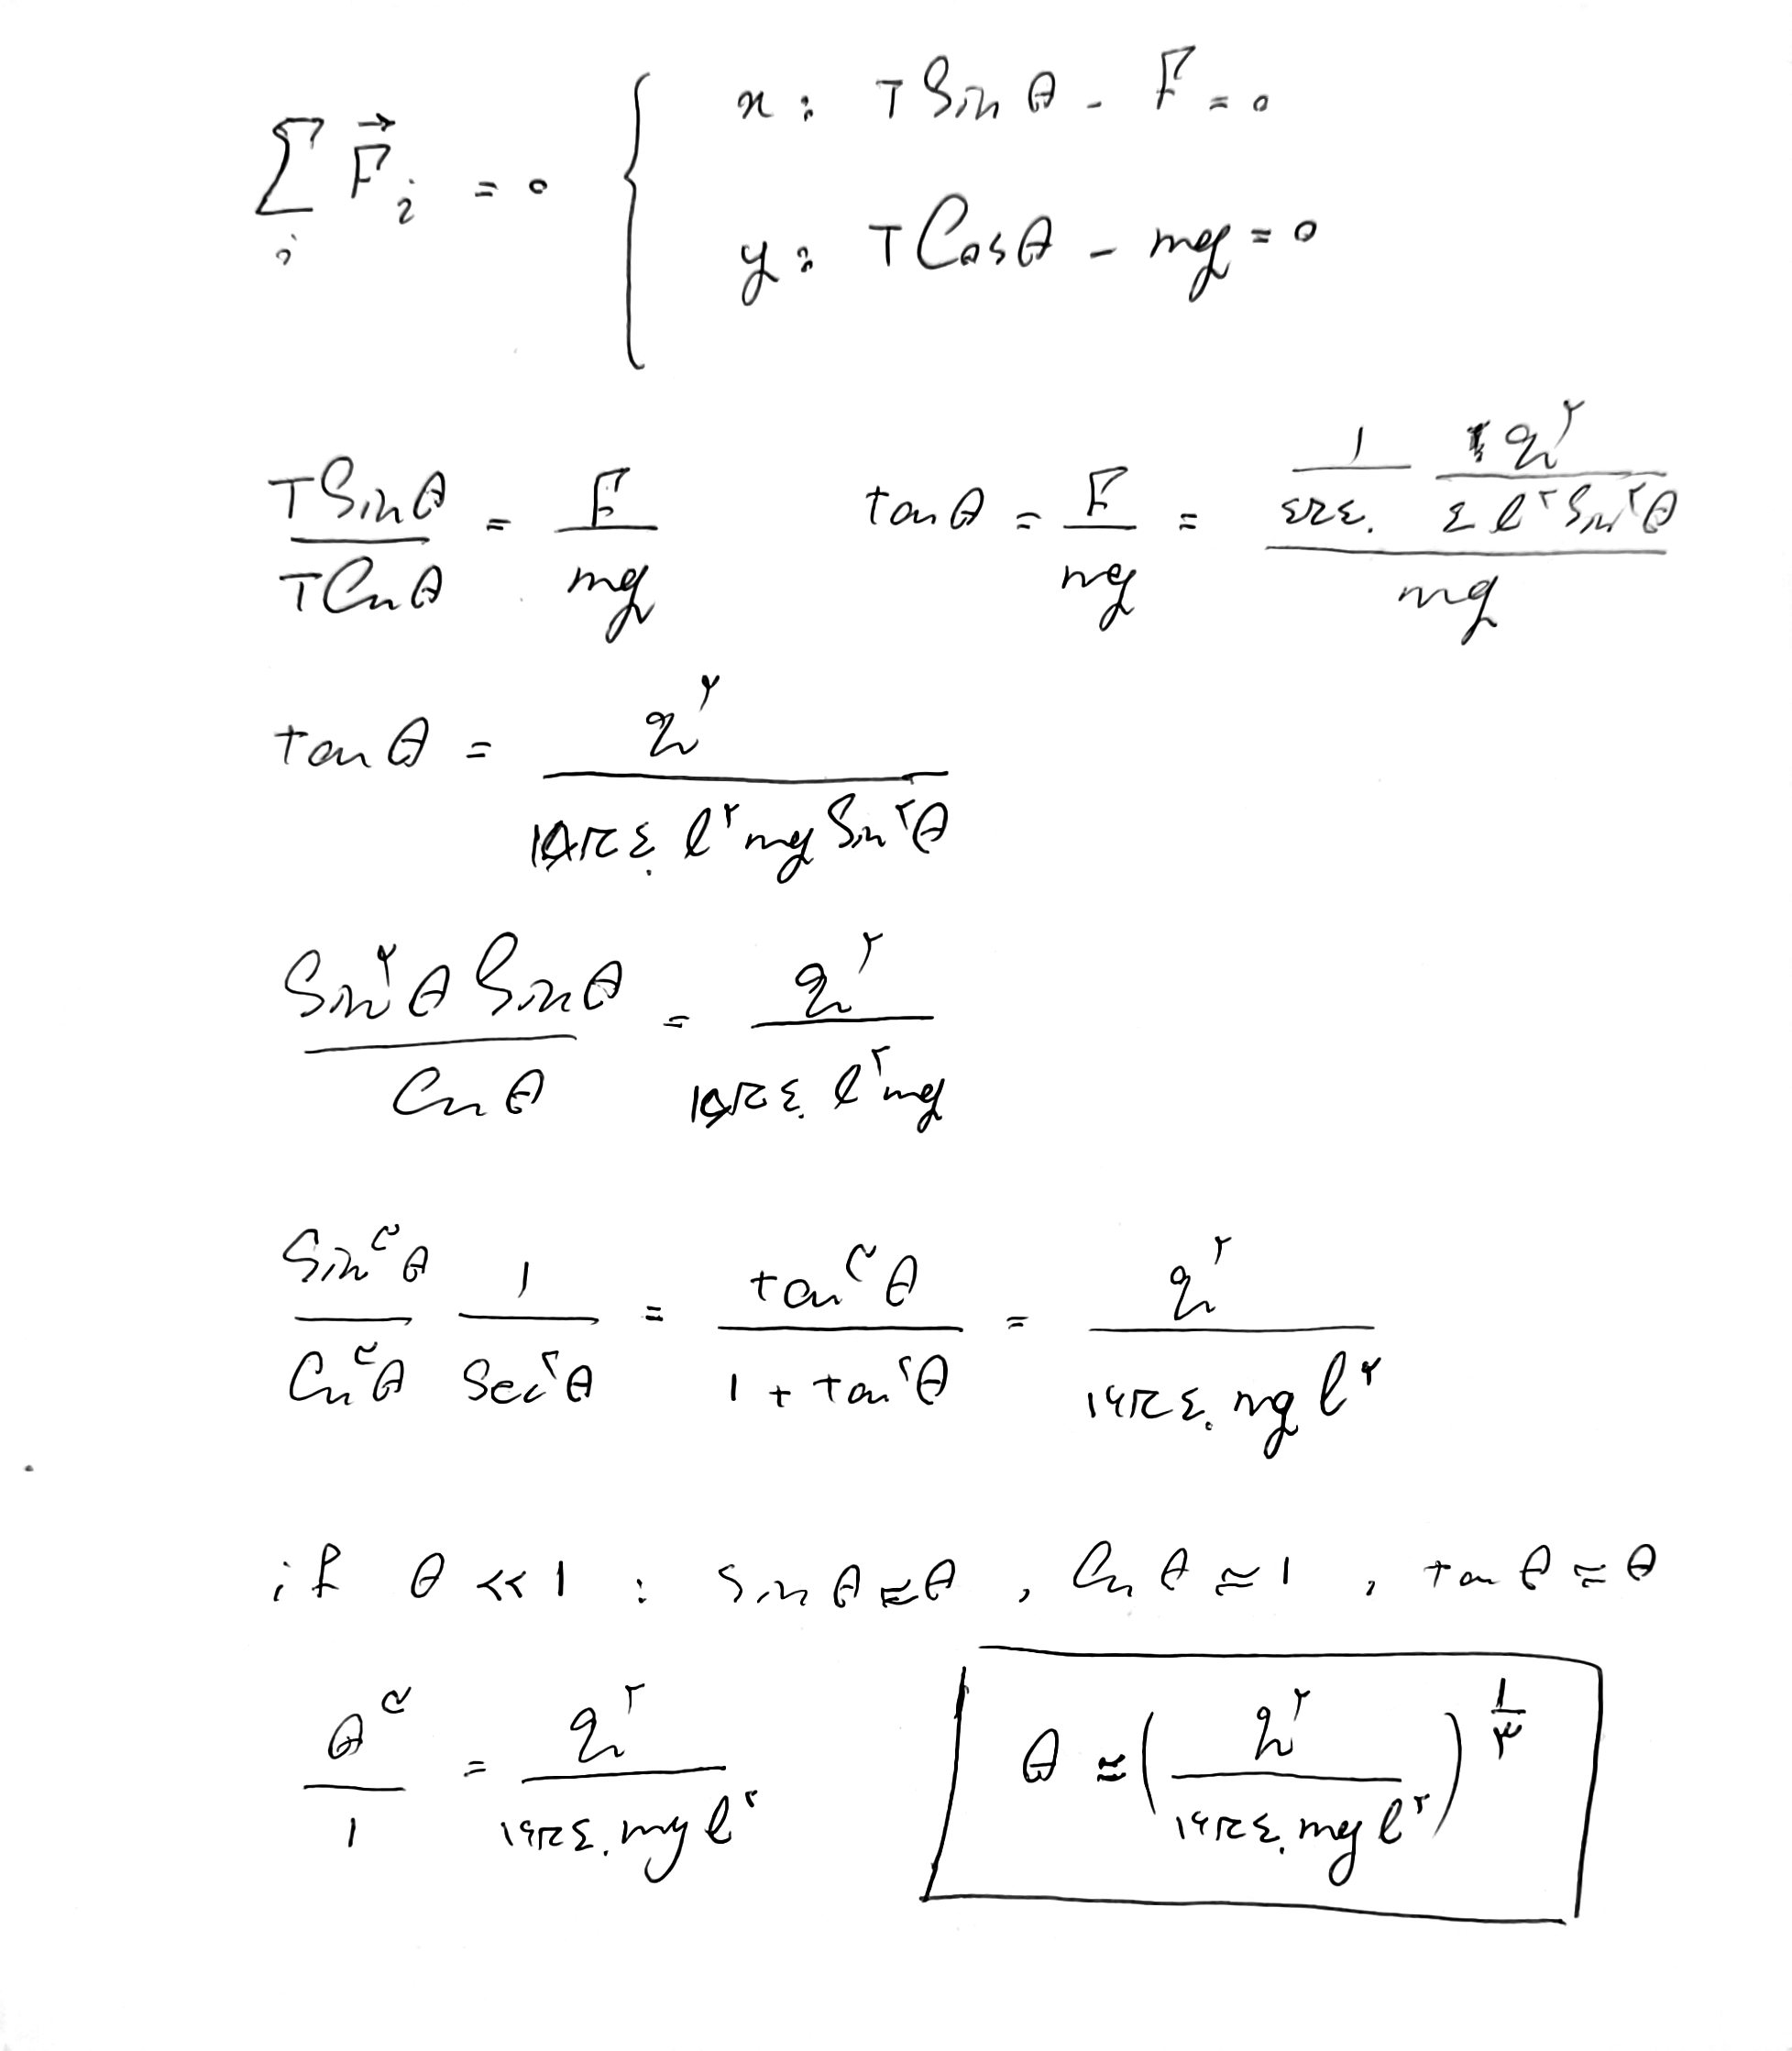
\includegraphics[width=0.6\textwidth]{2.1-so.jpg}
\end{figure}

\begin{figure}[h!]
 \centering
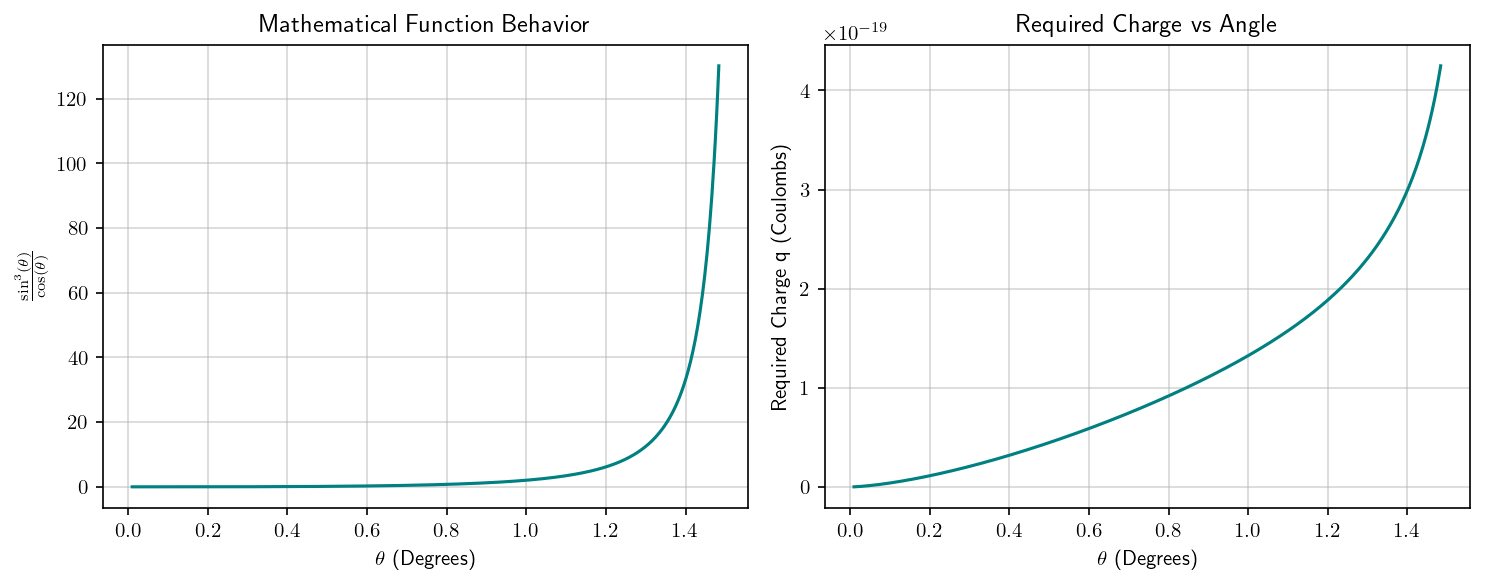
\includegraphics[width=0.8\textwidth]{plt_(2-1).png}
\end{figure}

\subsection{}

الف) 
\[ F = \frac{q_1 q_2}{4\pi \epsilon_0 r^2} = \frac{-0.8 \times 10^{-18}}{4\pi \times 8.854 \times 10^{-12} \times 16 \times 10^{-4}} N = -0.000004493871219 N = -0.45 \times 10^{-5} N \]

ب)
\[ q_{\text{new}} = \frac{q_1 + q_2}{2} = 0.8 \times 10^{-9} \]
\[ F = \frac{q_1 q_2}{4\pi \epsilon_0 r^2} = \frac{0.64 \times 10^{-18}}{4\pi \times 8.854 \times 10^{-12} \times 16 \times 10^{-4}} N = 0.000003595096975 N = 0.36 \times 10^{-5} N \]

\subsection{}
\begin{figure}[h!]
 \centering
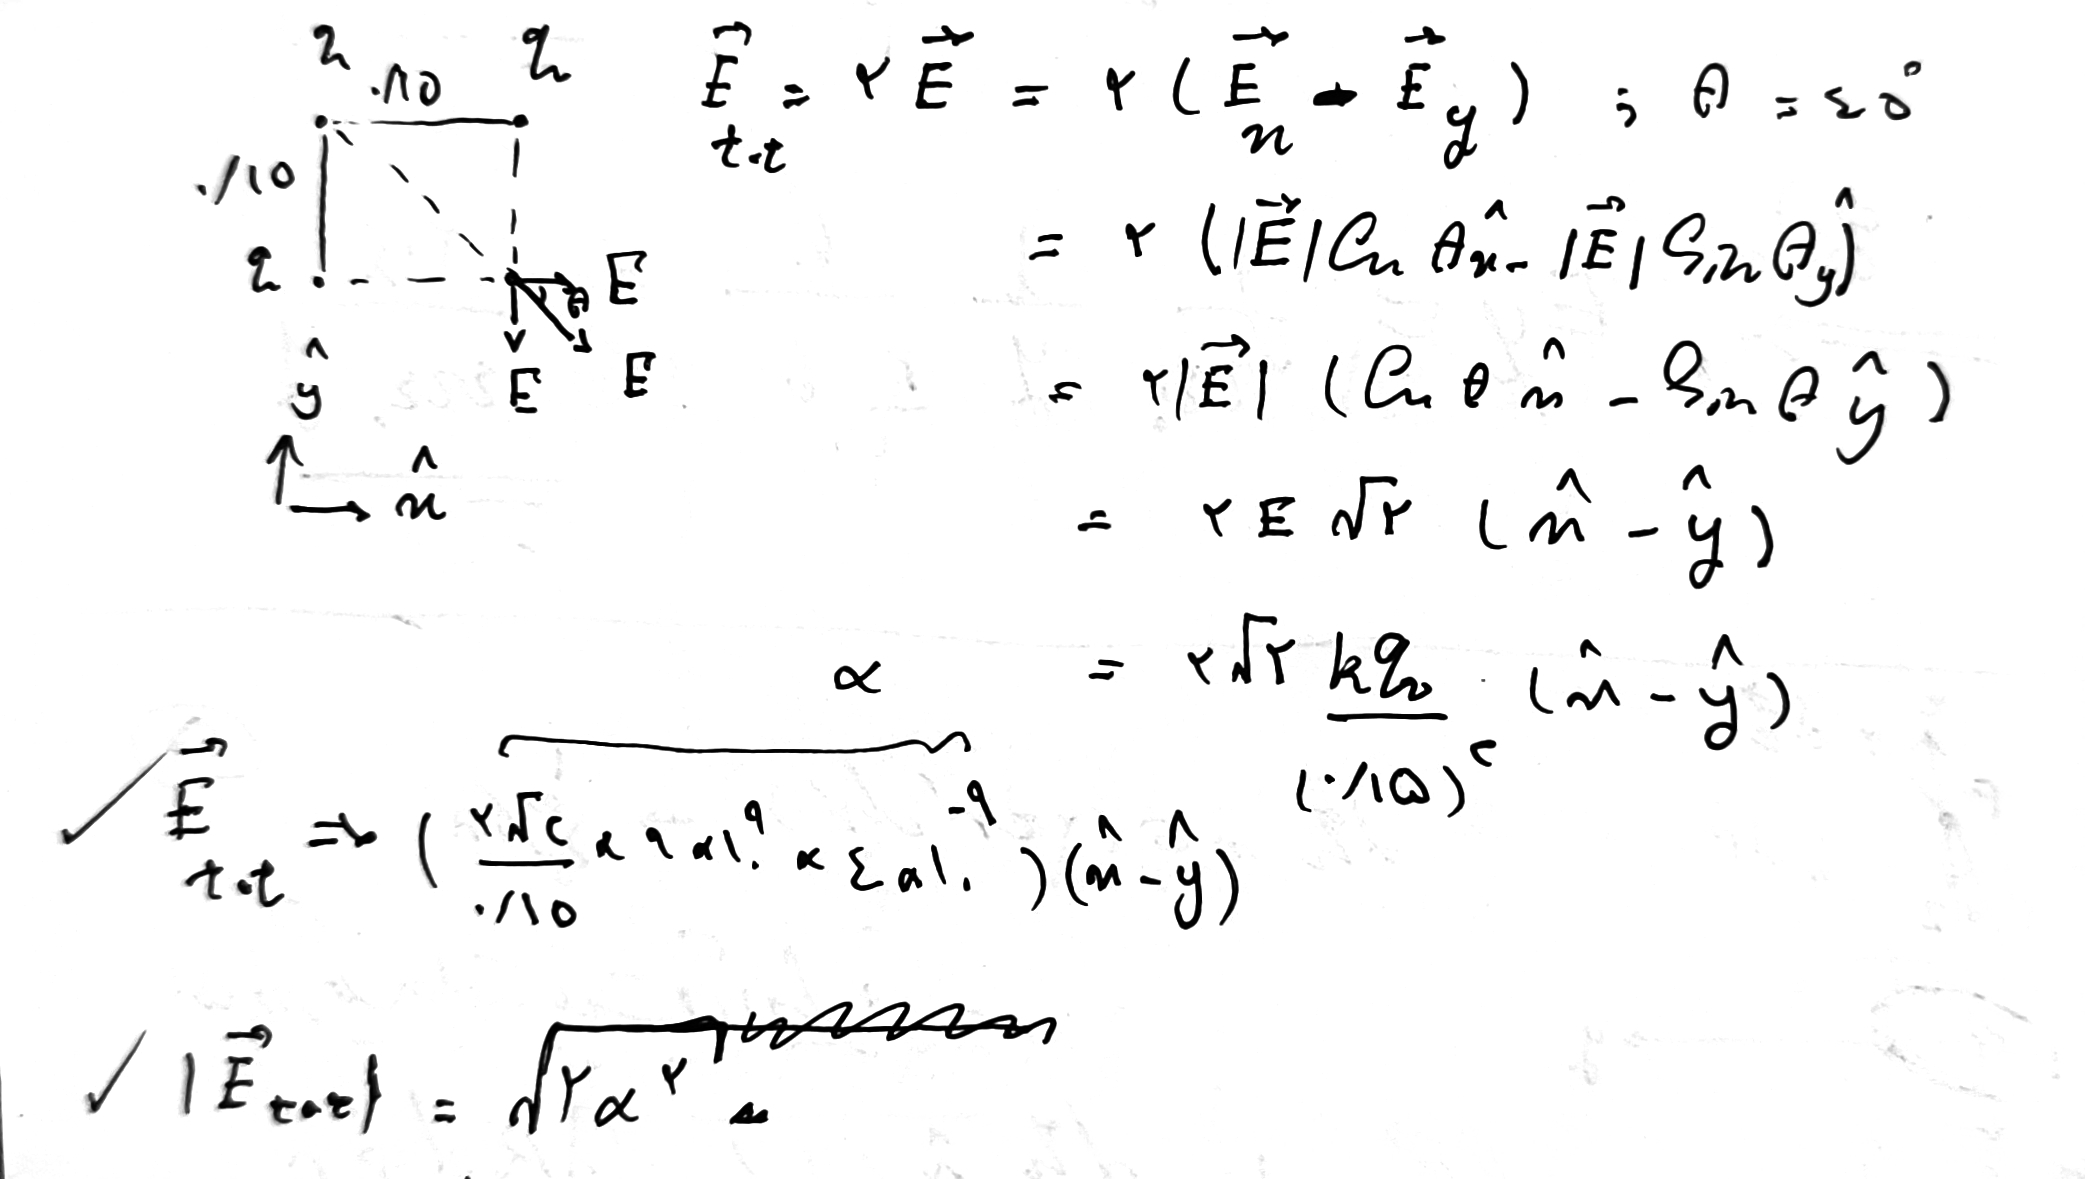
\includegraphics[width=1\textwidth]{2.3-so.jpg}
\end{figure}

\newpage
\subsection{}
\begin{figure}[h!]
 \centering
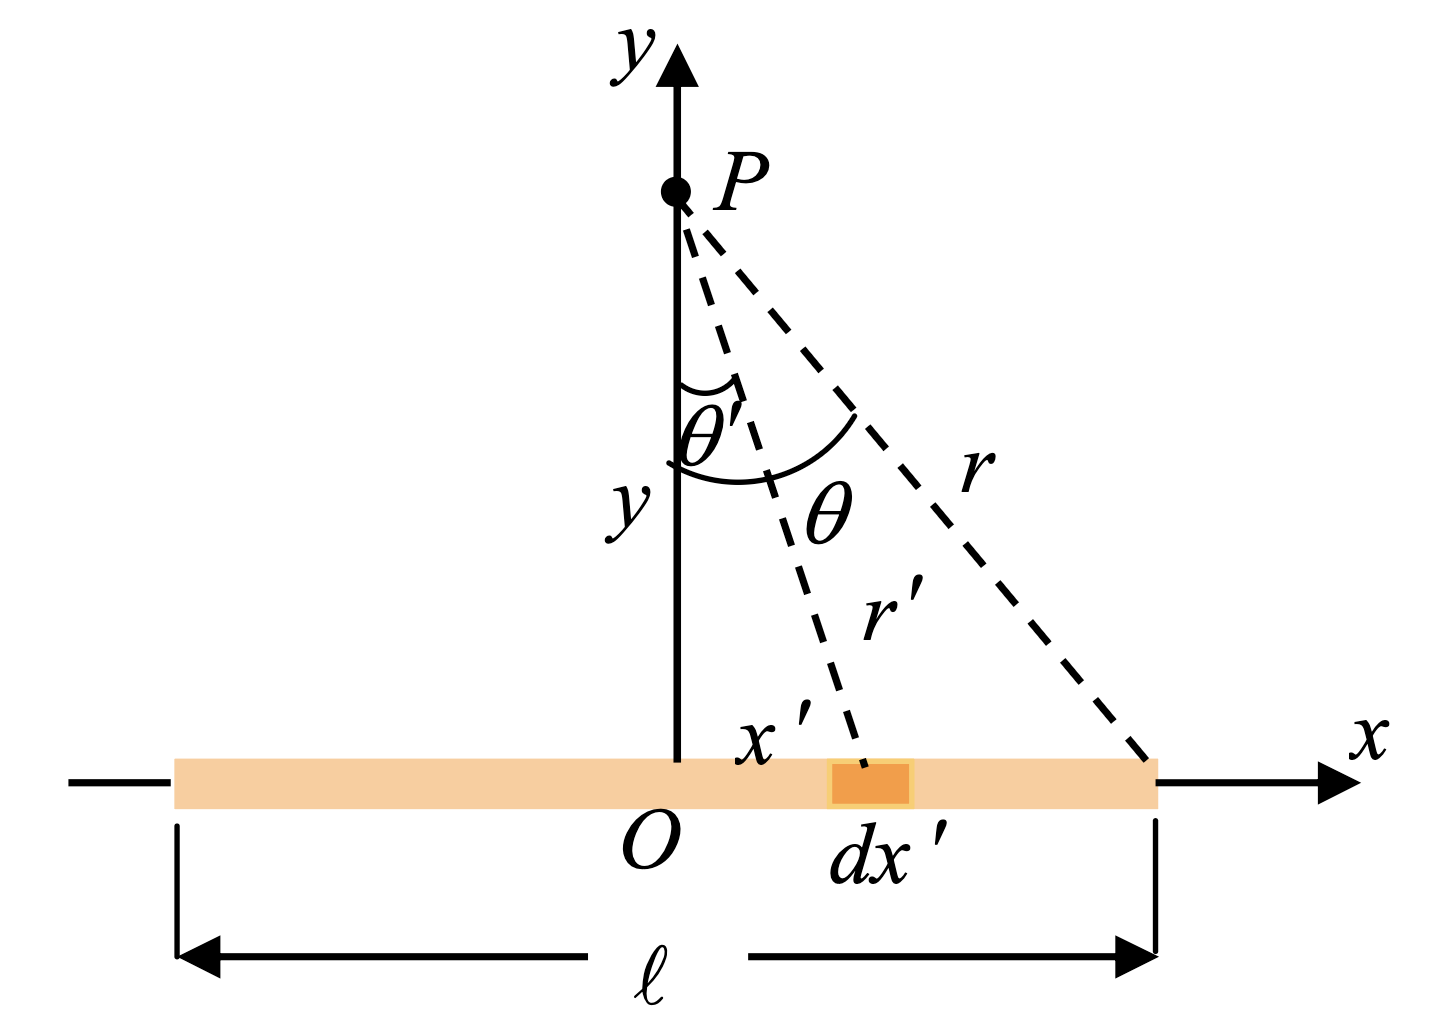
\includegraphics[width=0.4\textwidth]{2.4fig}
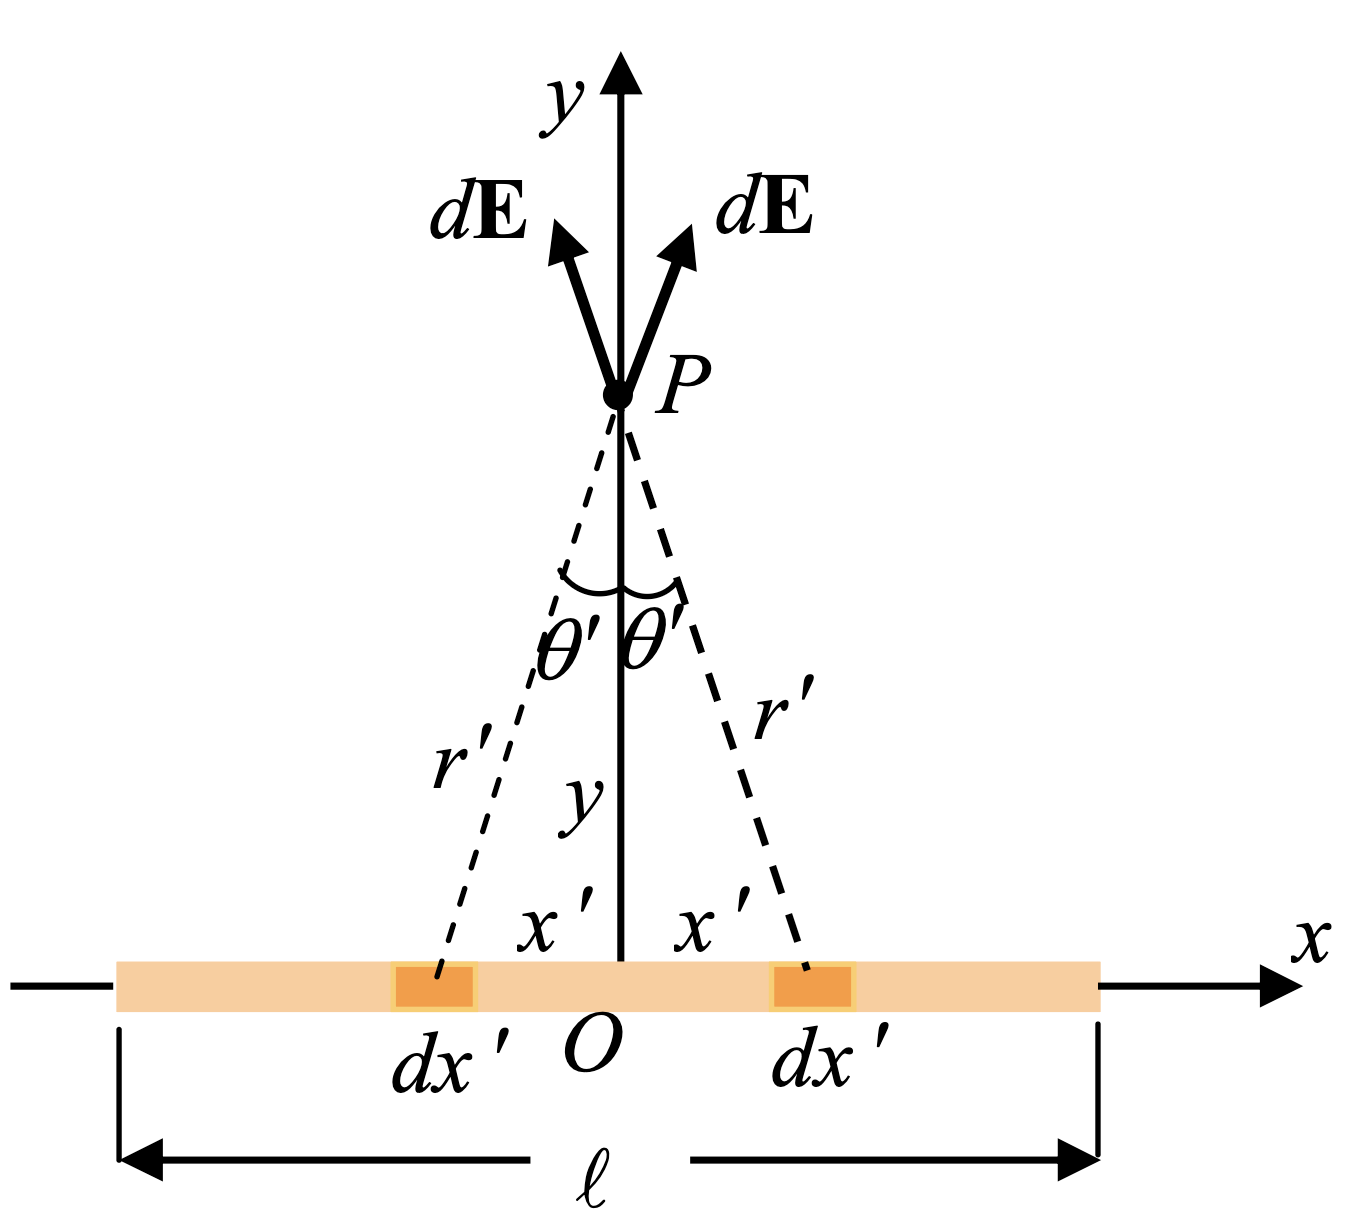
\includegraphics[width=0.4\textwidth]{2.4fig2}
\end{figure}
\begin{figure}[h!]
 \centering
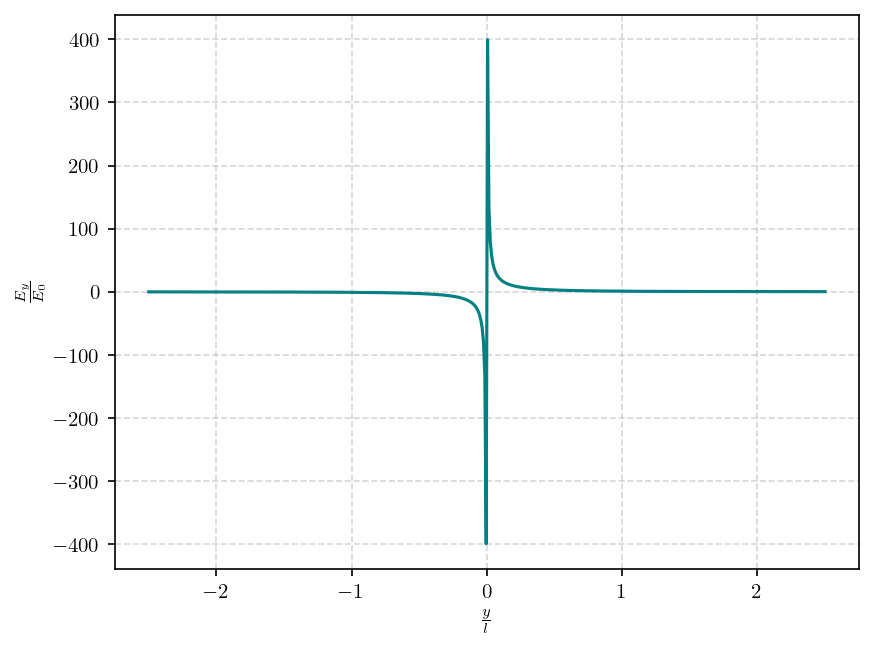
\includegraphics[width=0.8\textwidth]{2.4plot}
\end{figure}
\begin{figure}[h!]
 \centering
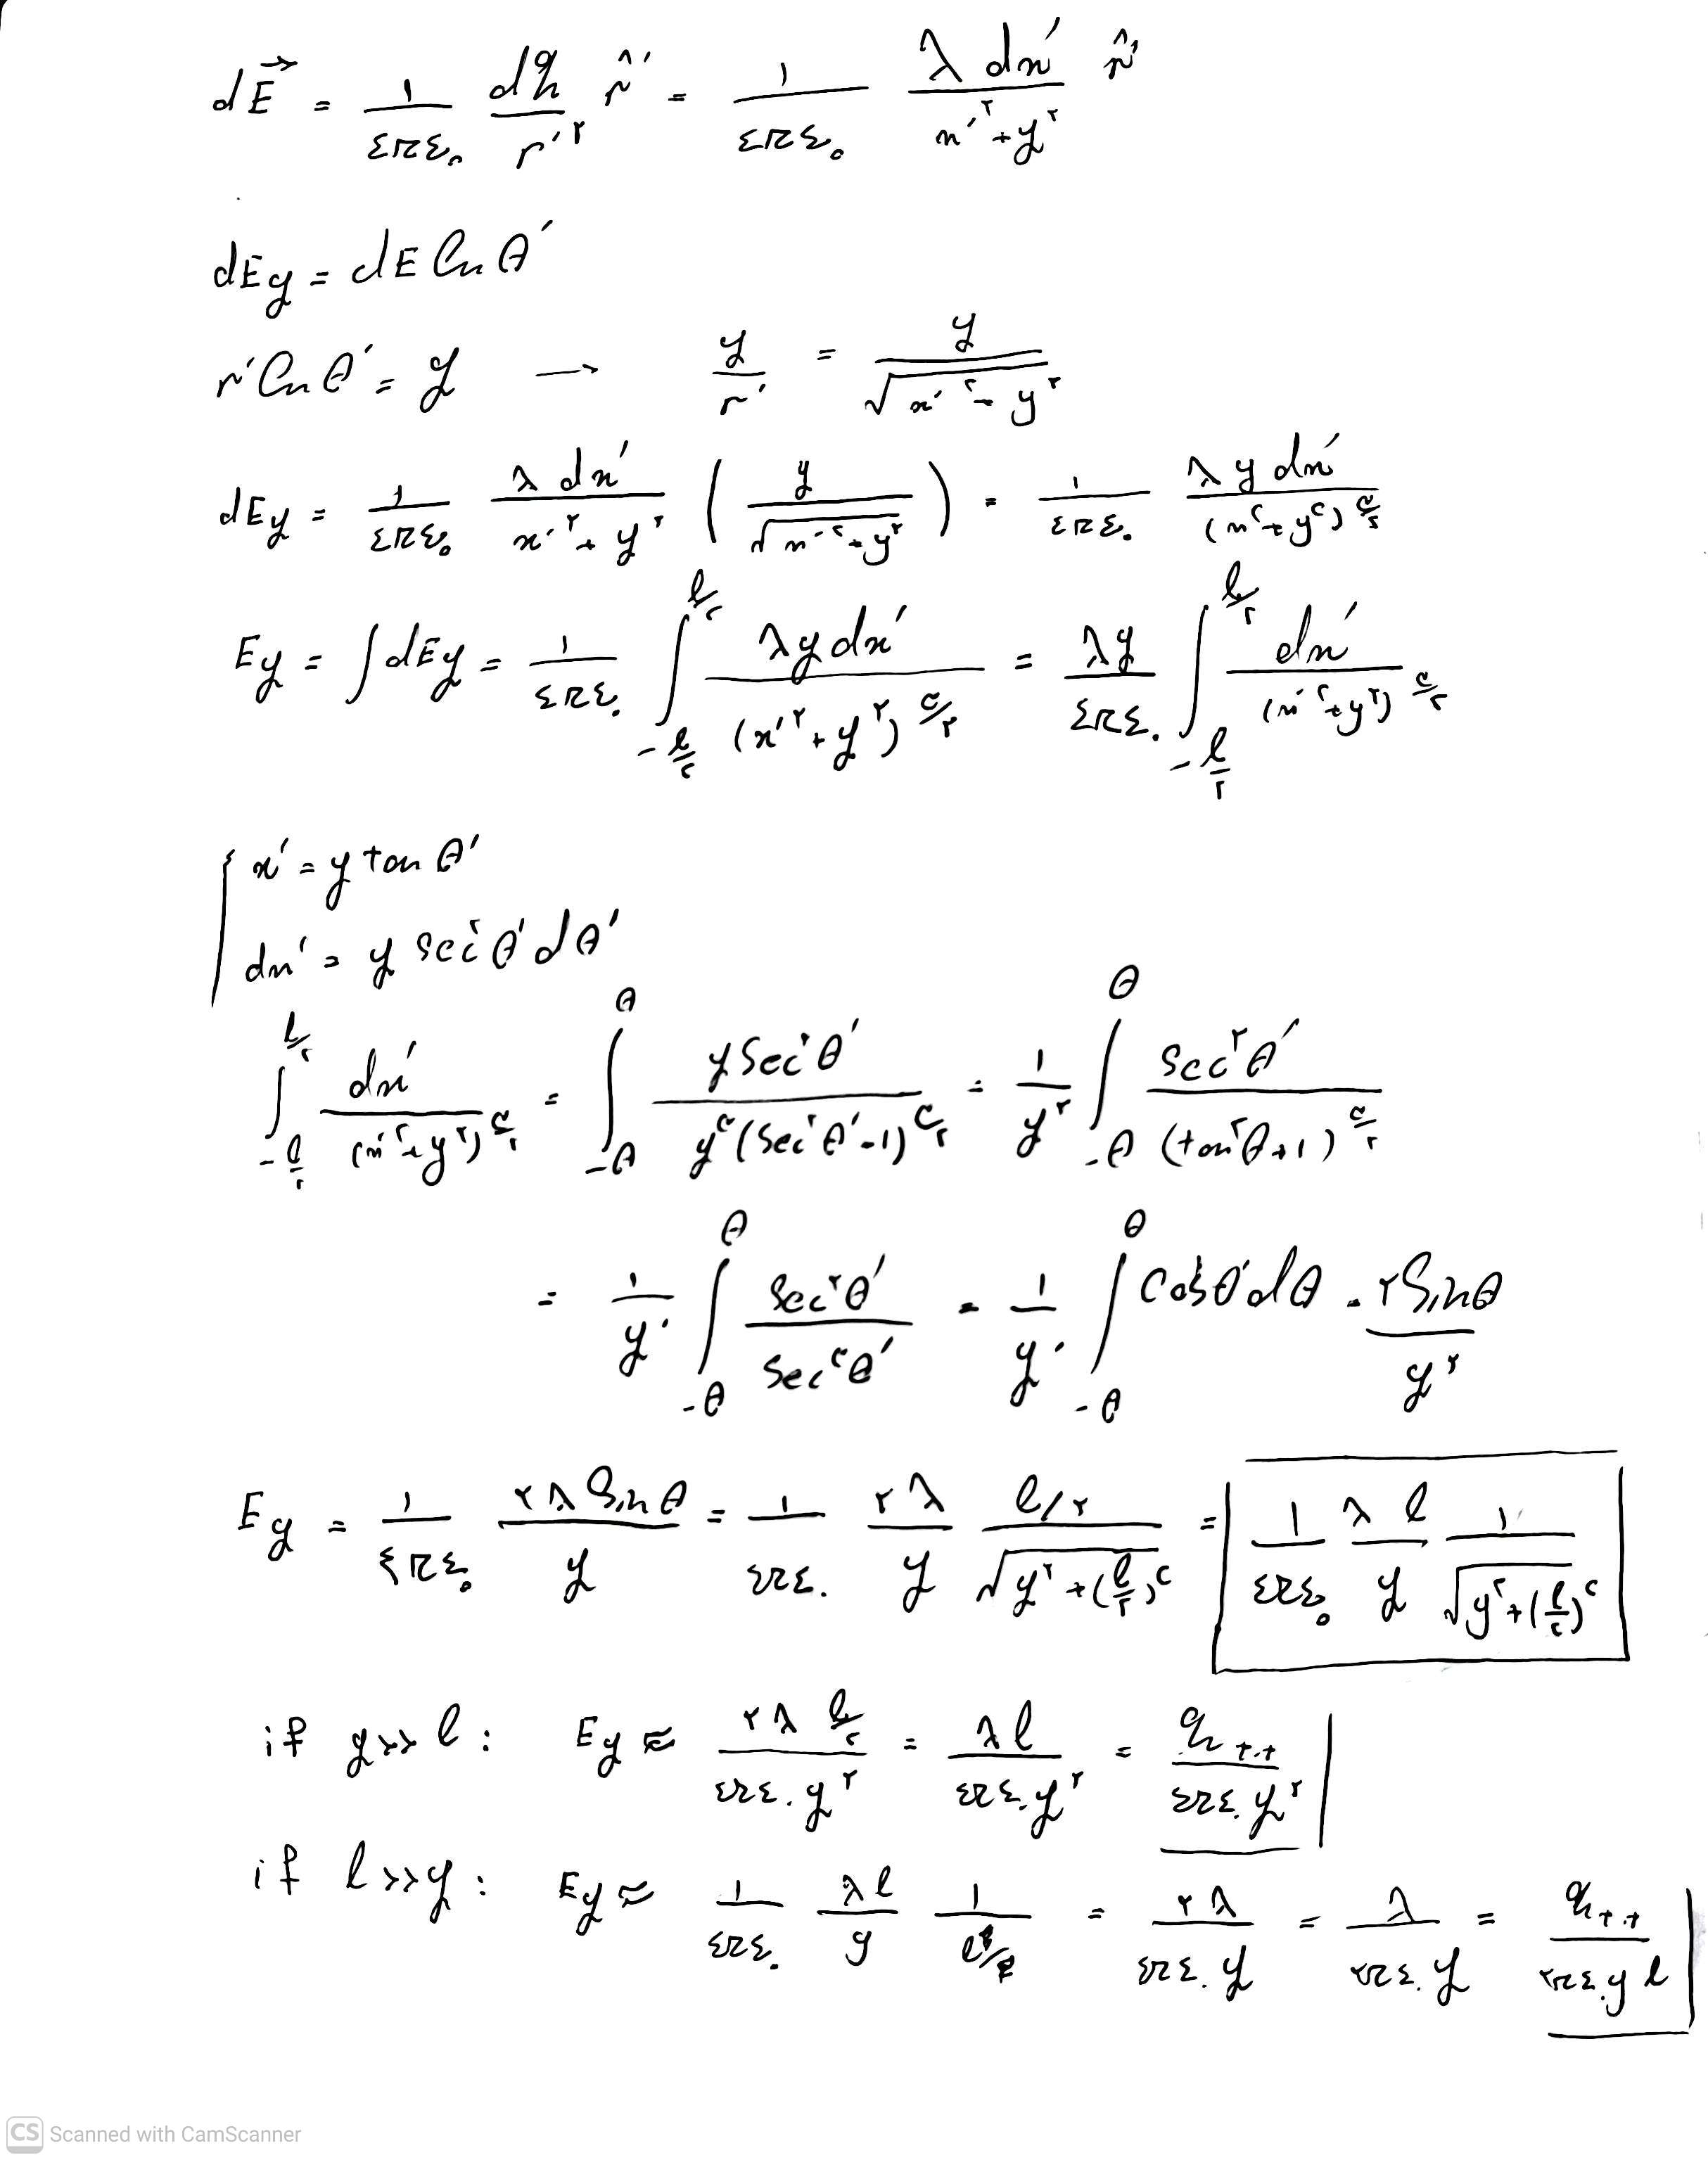
\includegraphics[width=1\textwidth]{2.4-so.jpg}
\end{figure}
\newpage
\subsection{}
الف)
\begin{figure}[h!]
\centering
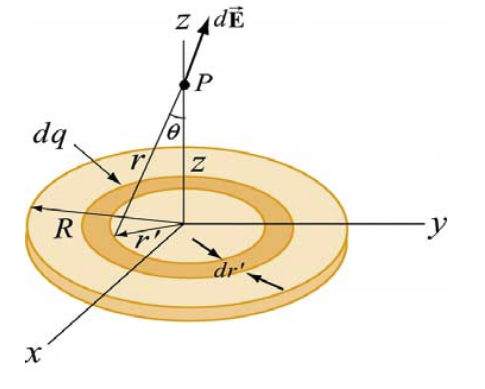
\includegraphics[width=0.3\textwidth]{2.5fig2}
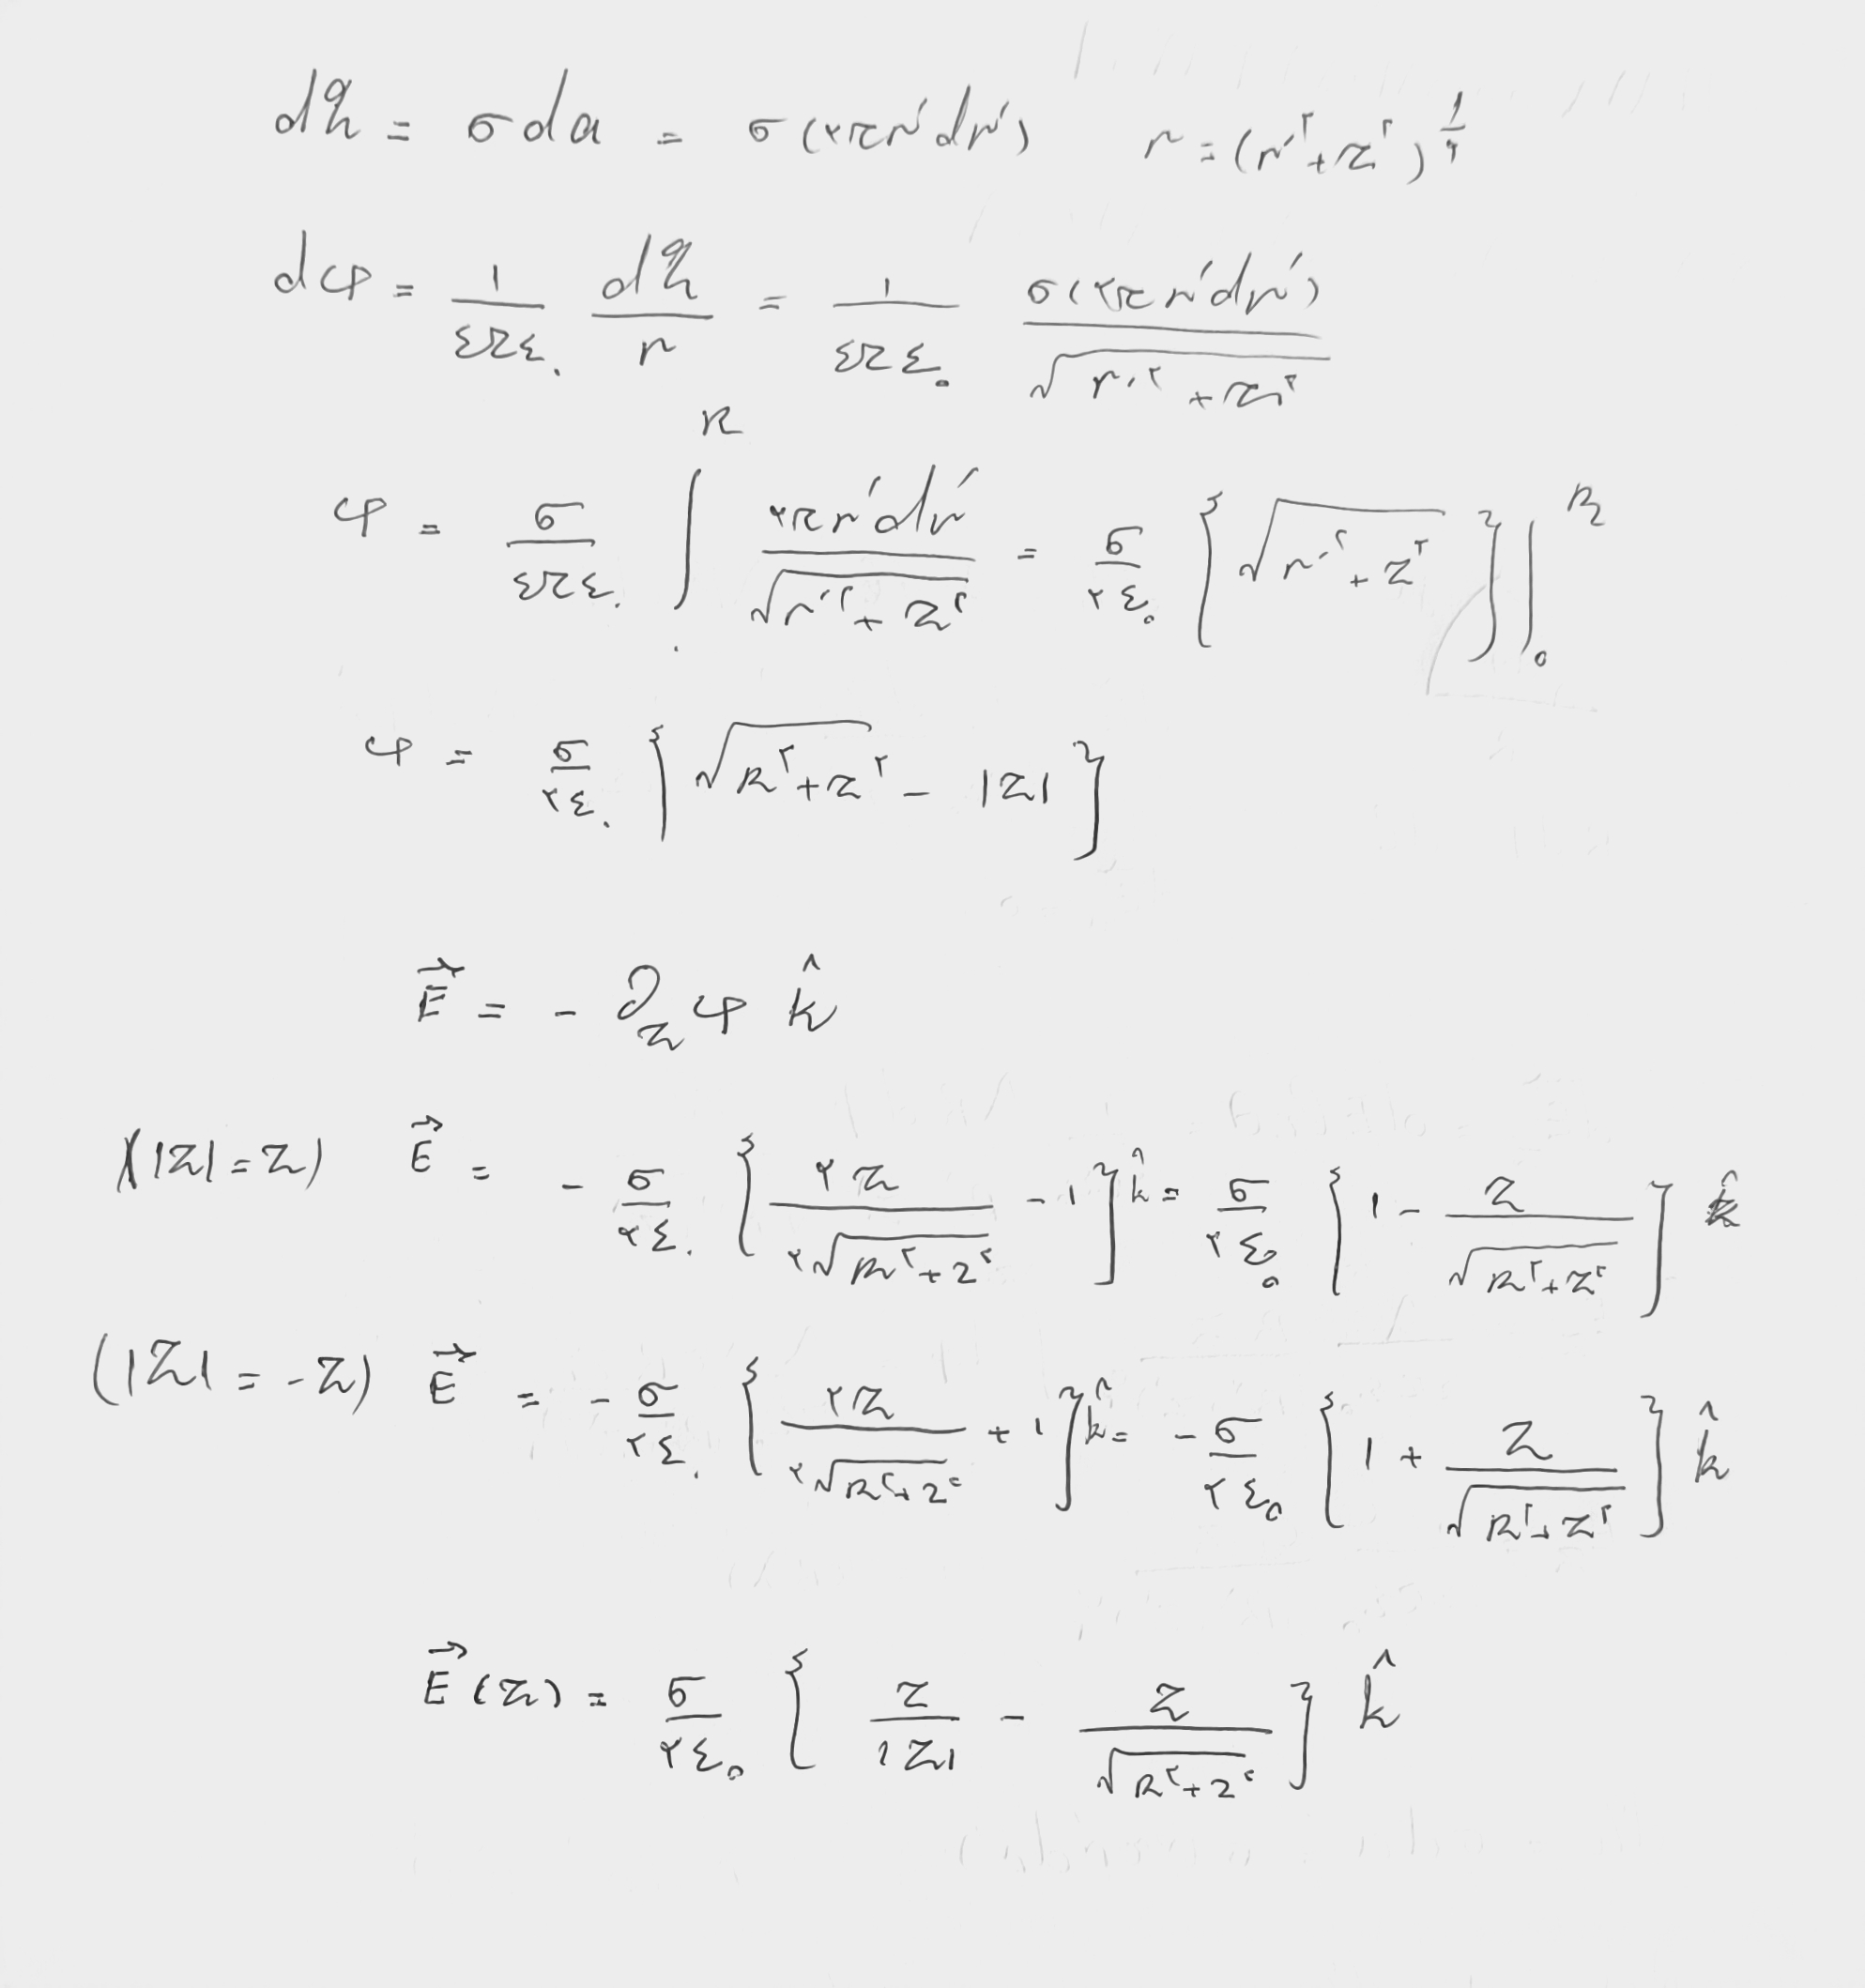
\includegraphics[width=0.5\textwidth]{2.5-so1.jpg}
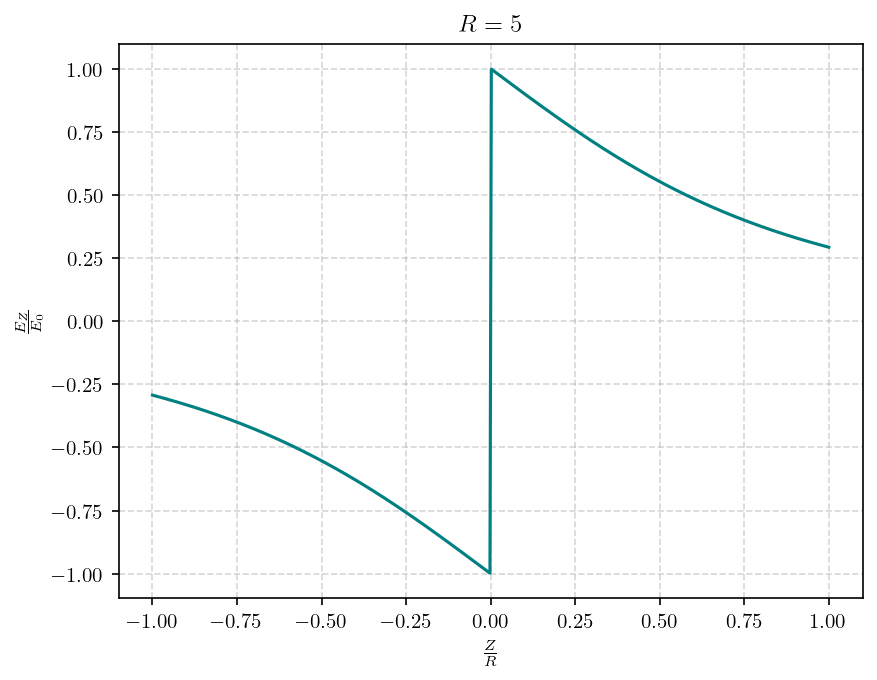
\includegraphics[width=0.7\textwidth]{2.5plt}
\end{figure}
\newpage
ب)
\begin{figure}[h!]
\centering
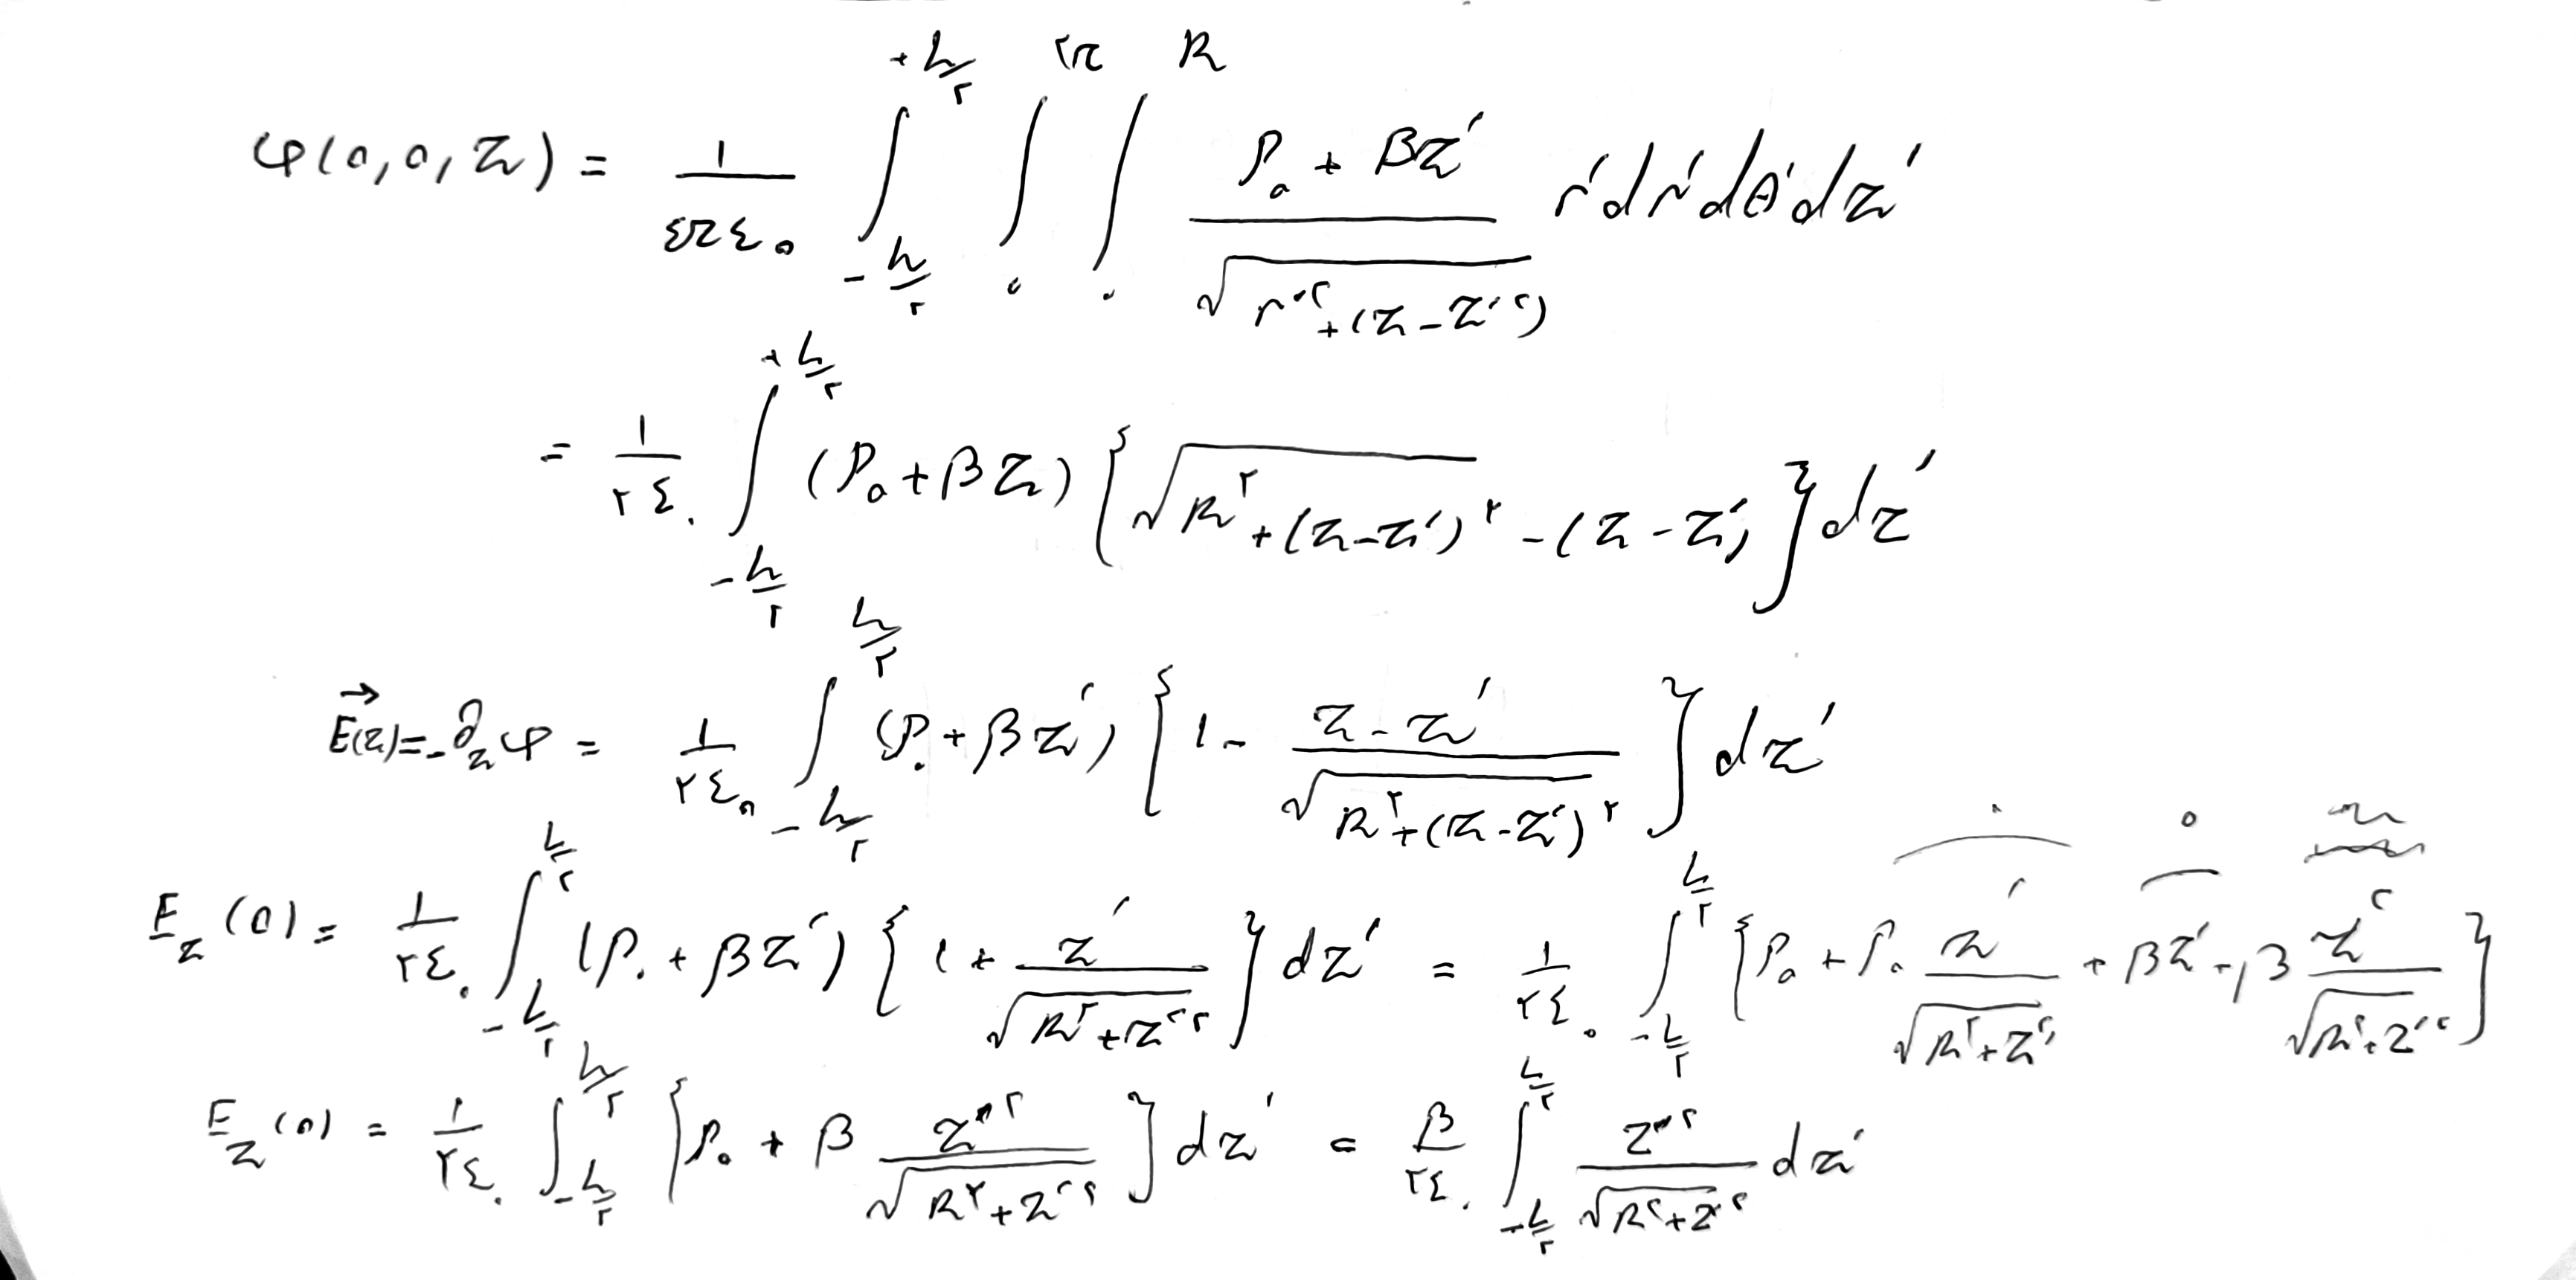
\includegraphics[width=1\textwidth]{2.5-so2.jpg}
\end{figure}
\subsection{}
\begin{figure}[h!]
\centering
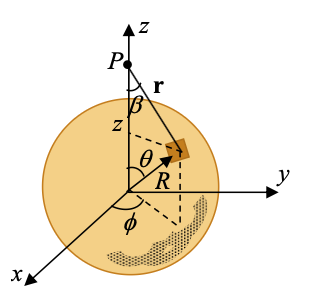
\includegraphics[width=0.3\textwidth]{2.6fig}
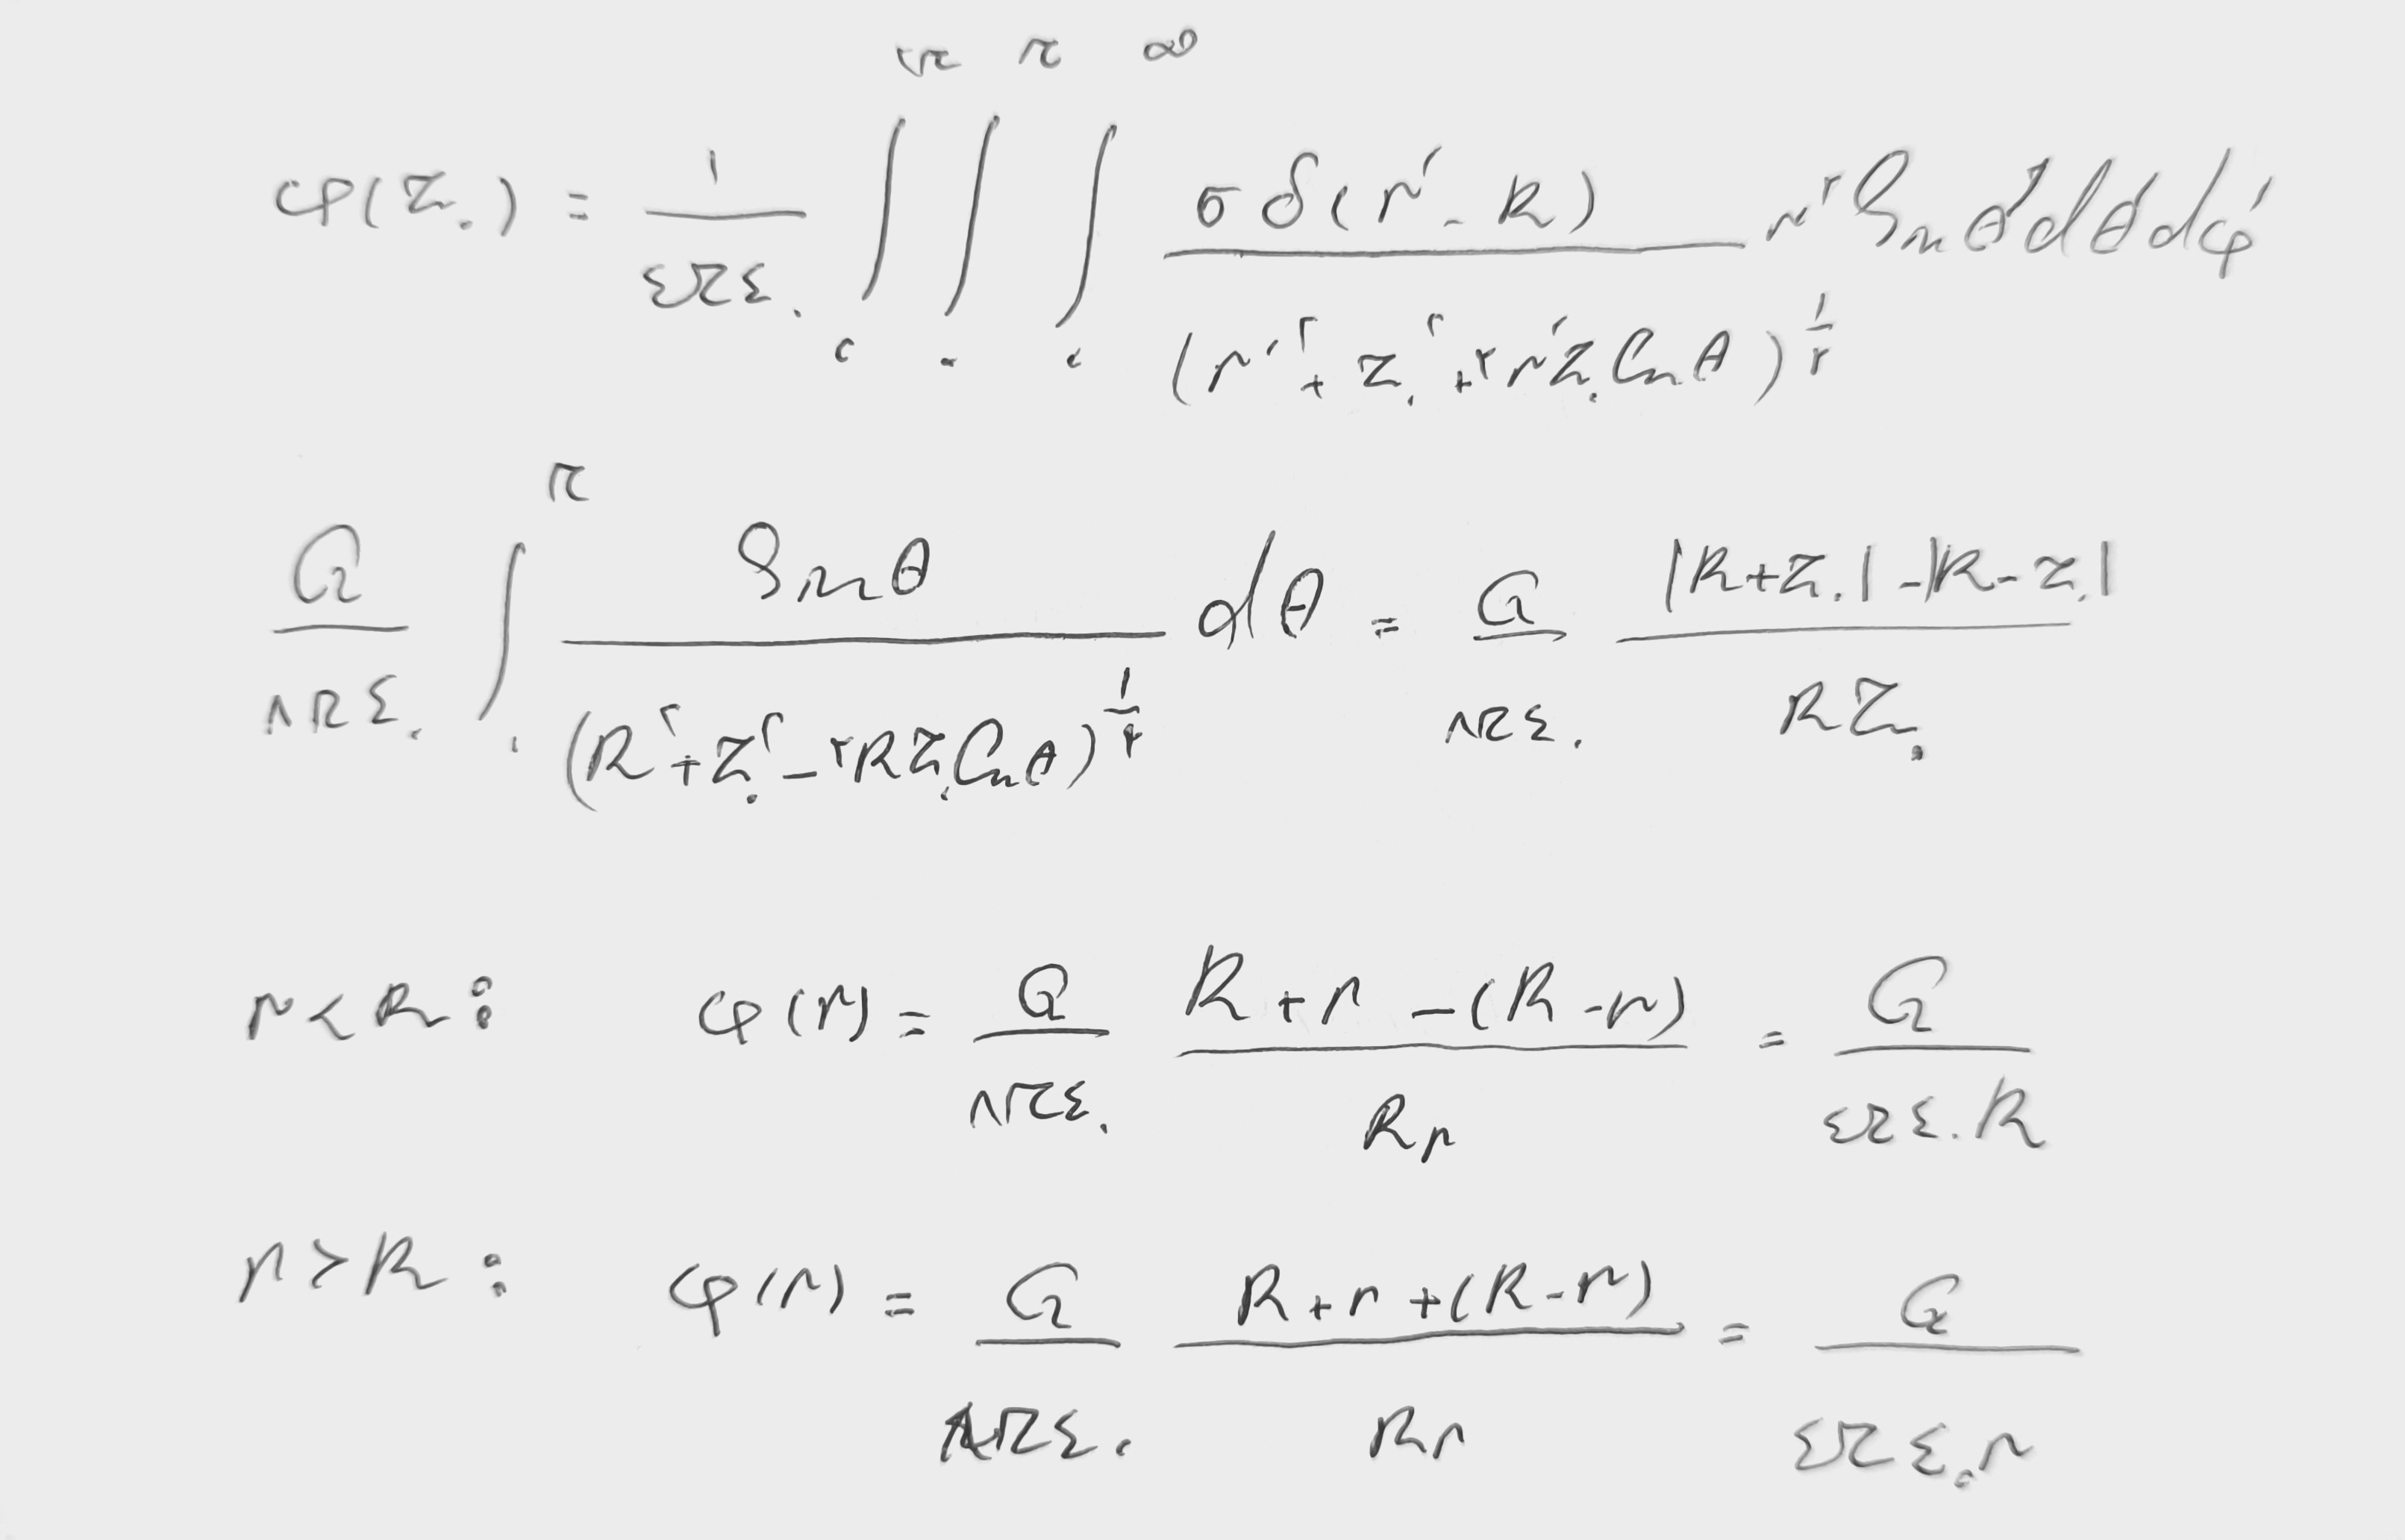
\includegraphics[width=0.6\textwidth]{2.6-so}
\end{figure}

\newpage
\subsection{}
\begin{figure}[h!]
\centering
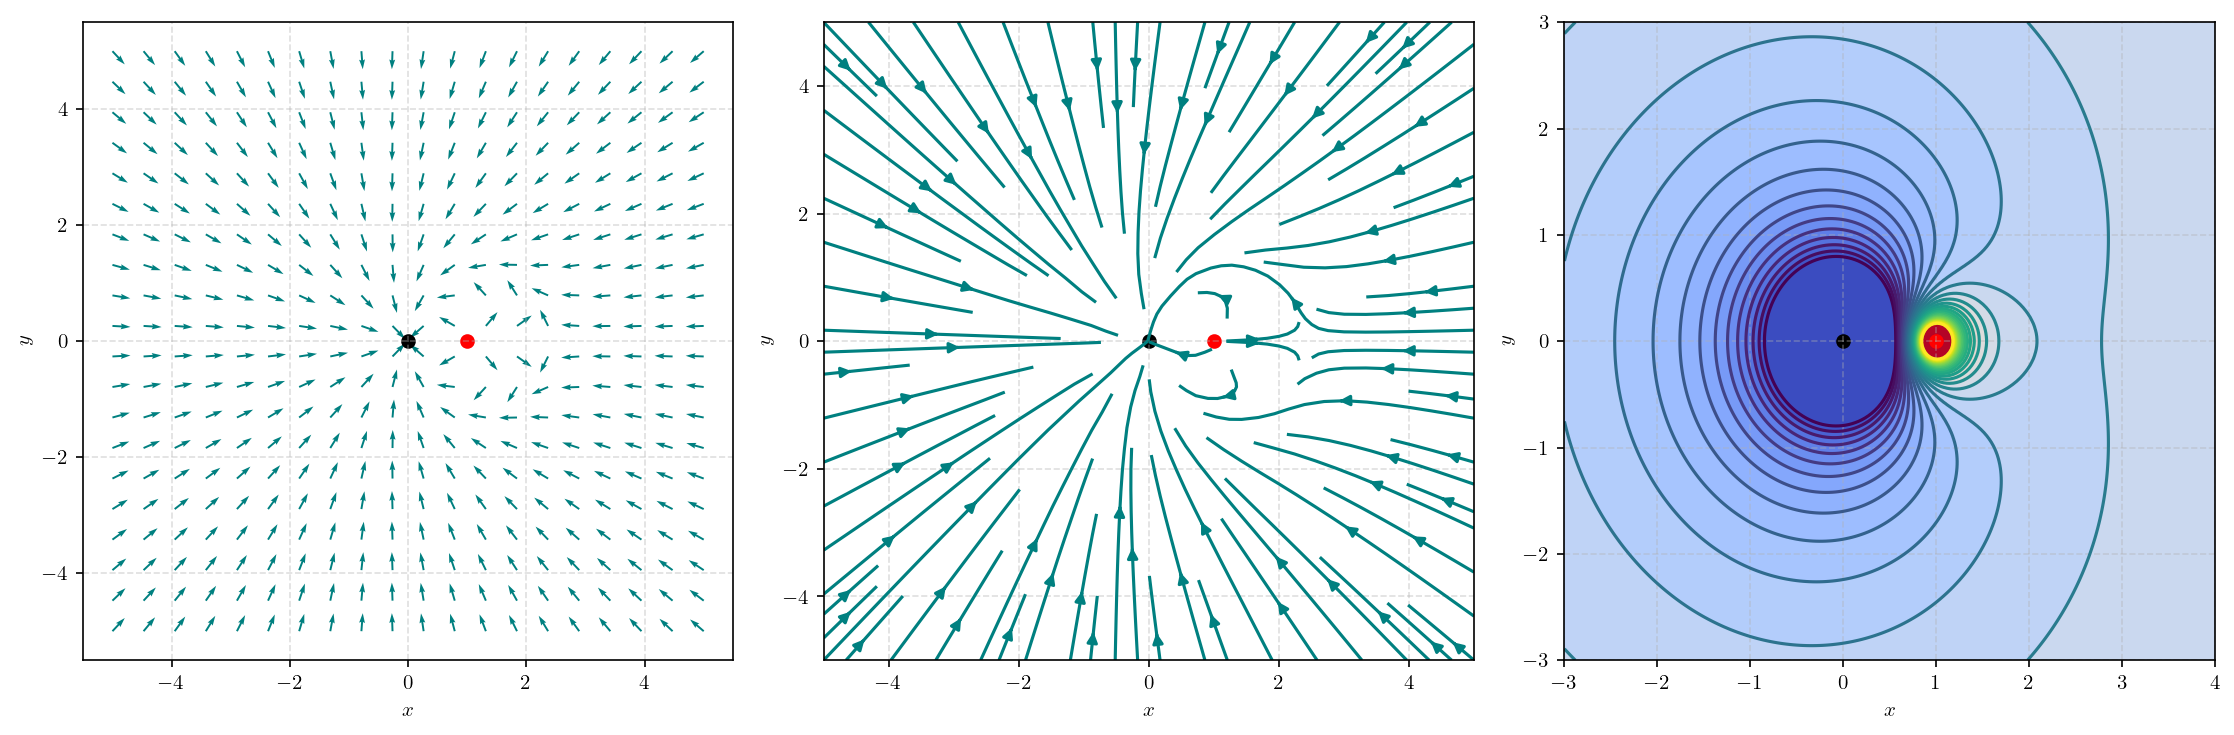
\includegraphics[width=1\textwidth]{2.7plt}
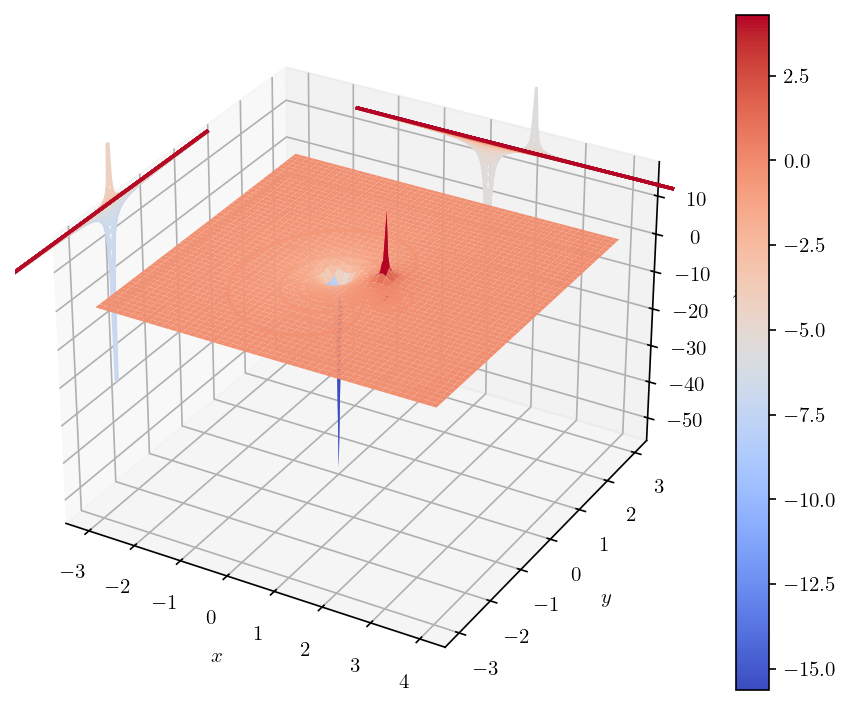
\includegraphics[width=0.5\textwidth]{2.7plt3D}
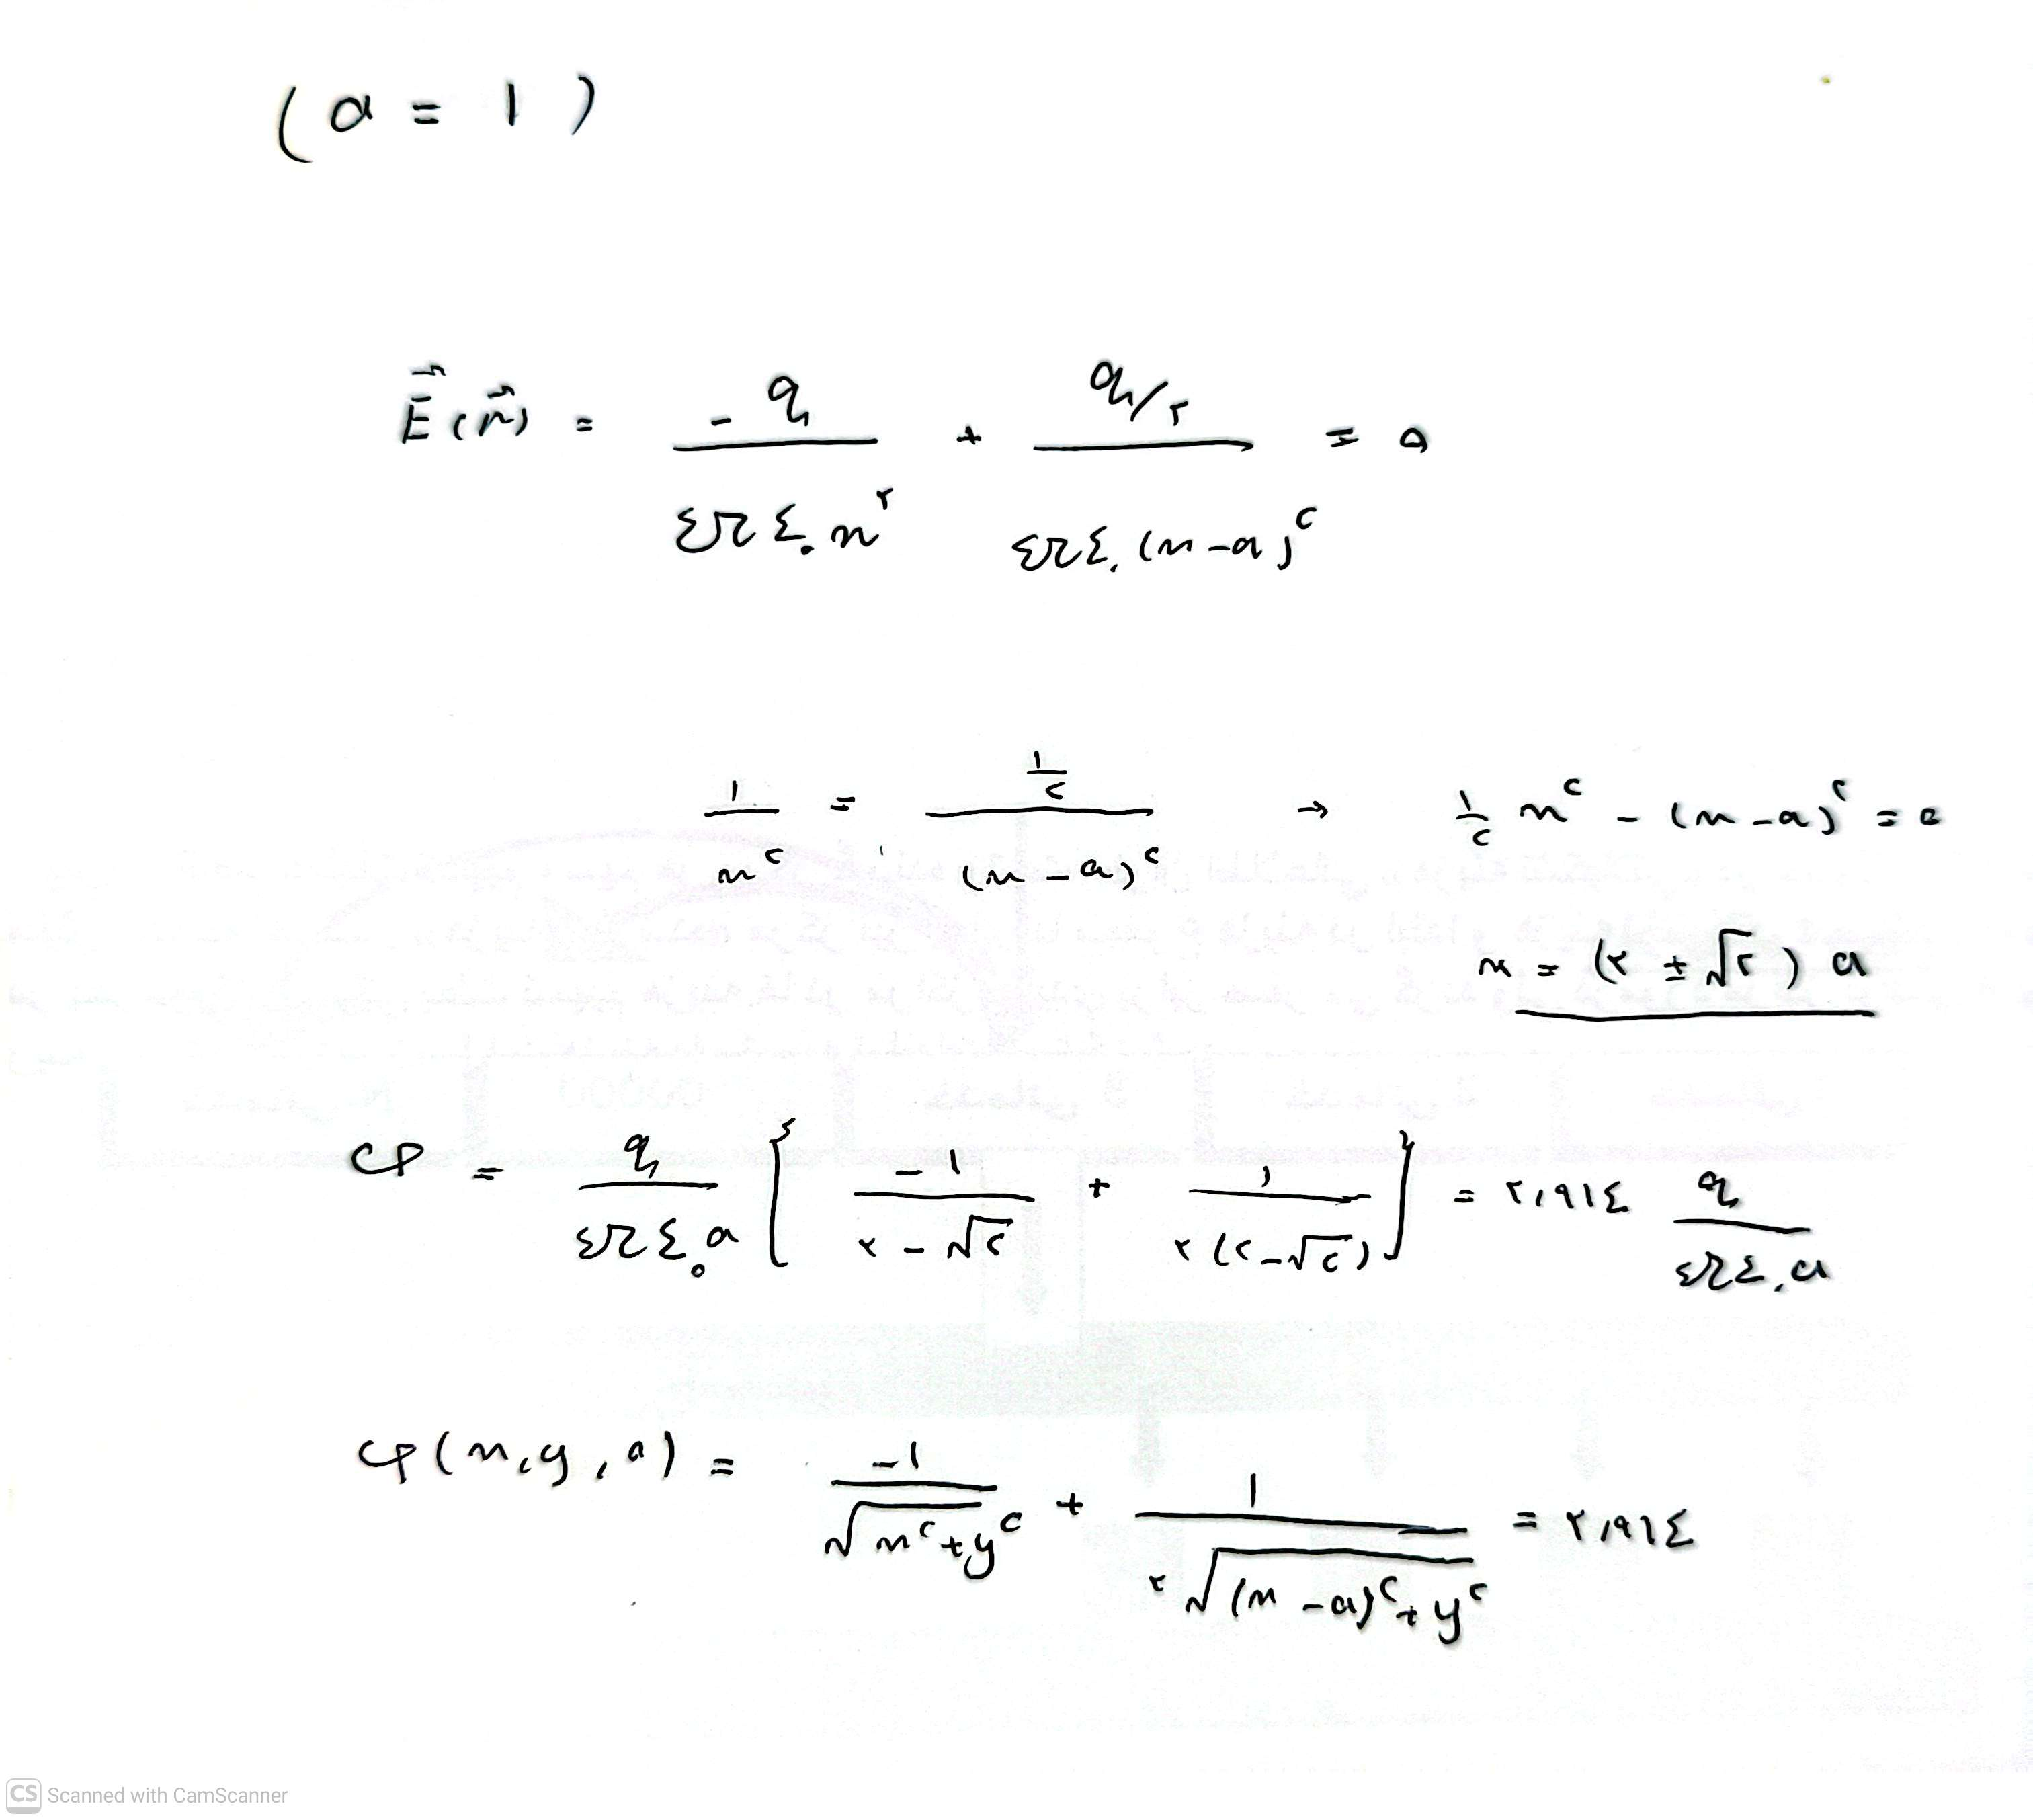
\includegraphics[width=0.5\textwidth]{2.7-so}
\end{figure}

\subsection{}
\begin{figure}[h!]
\centering
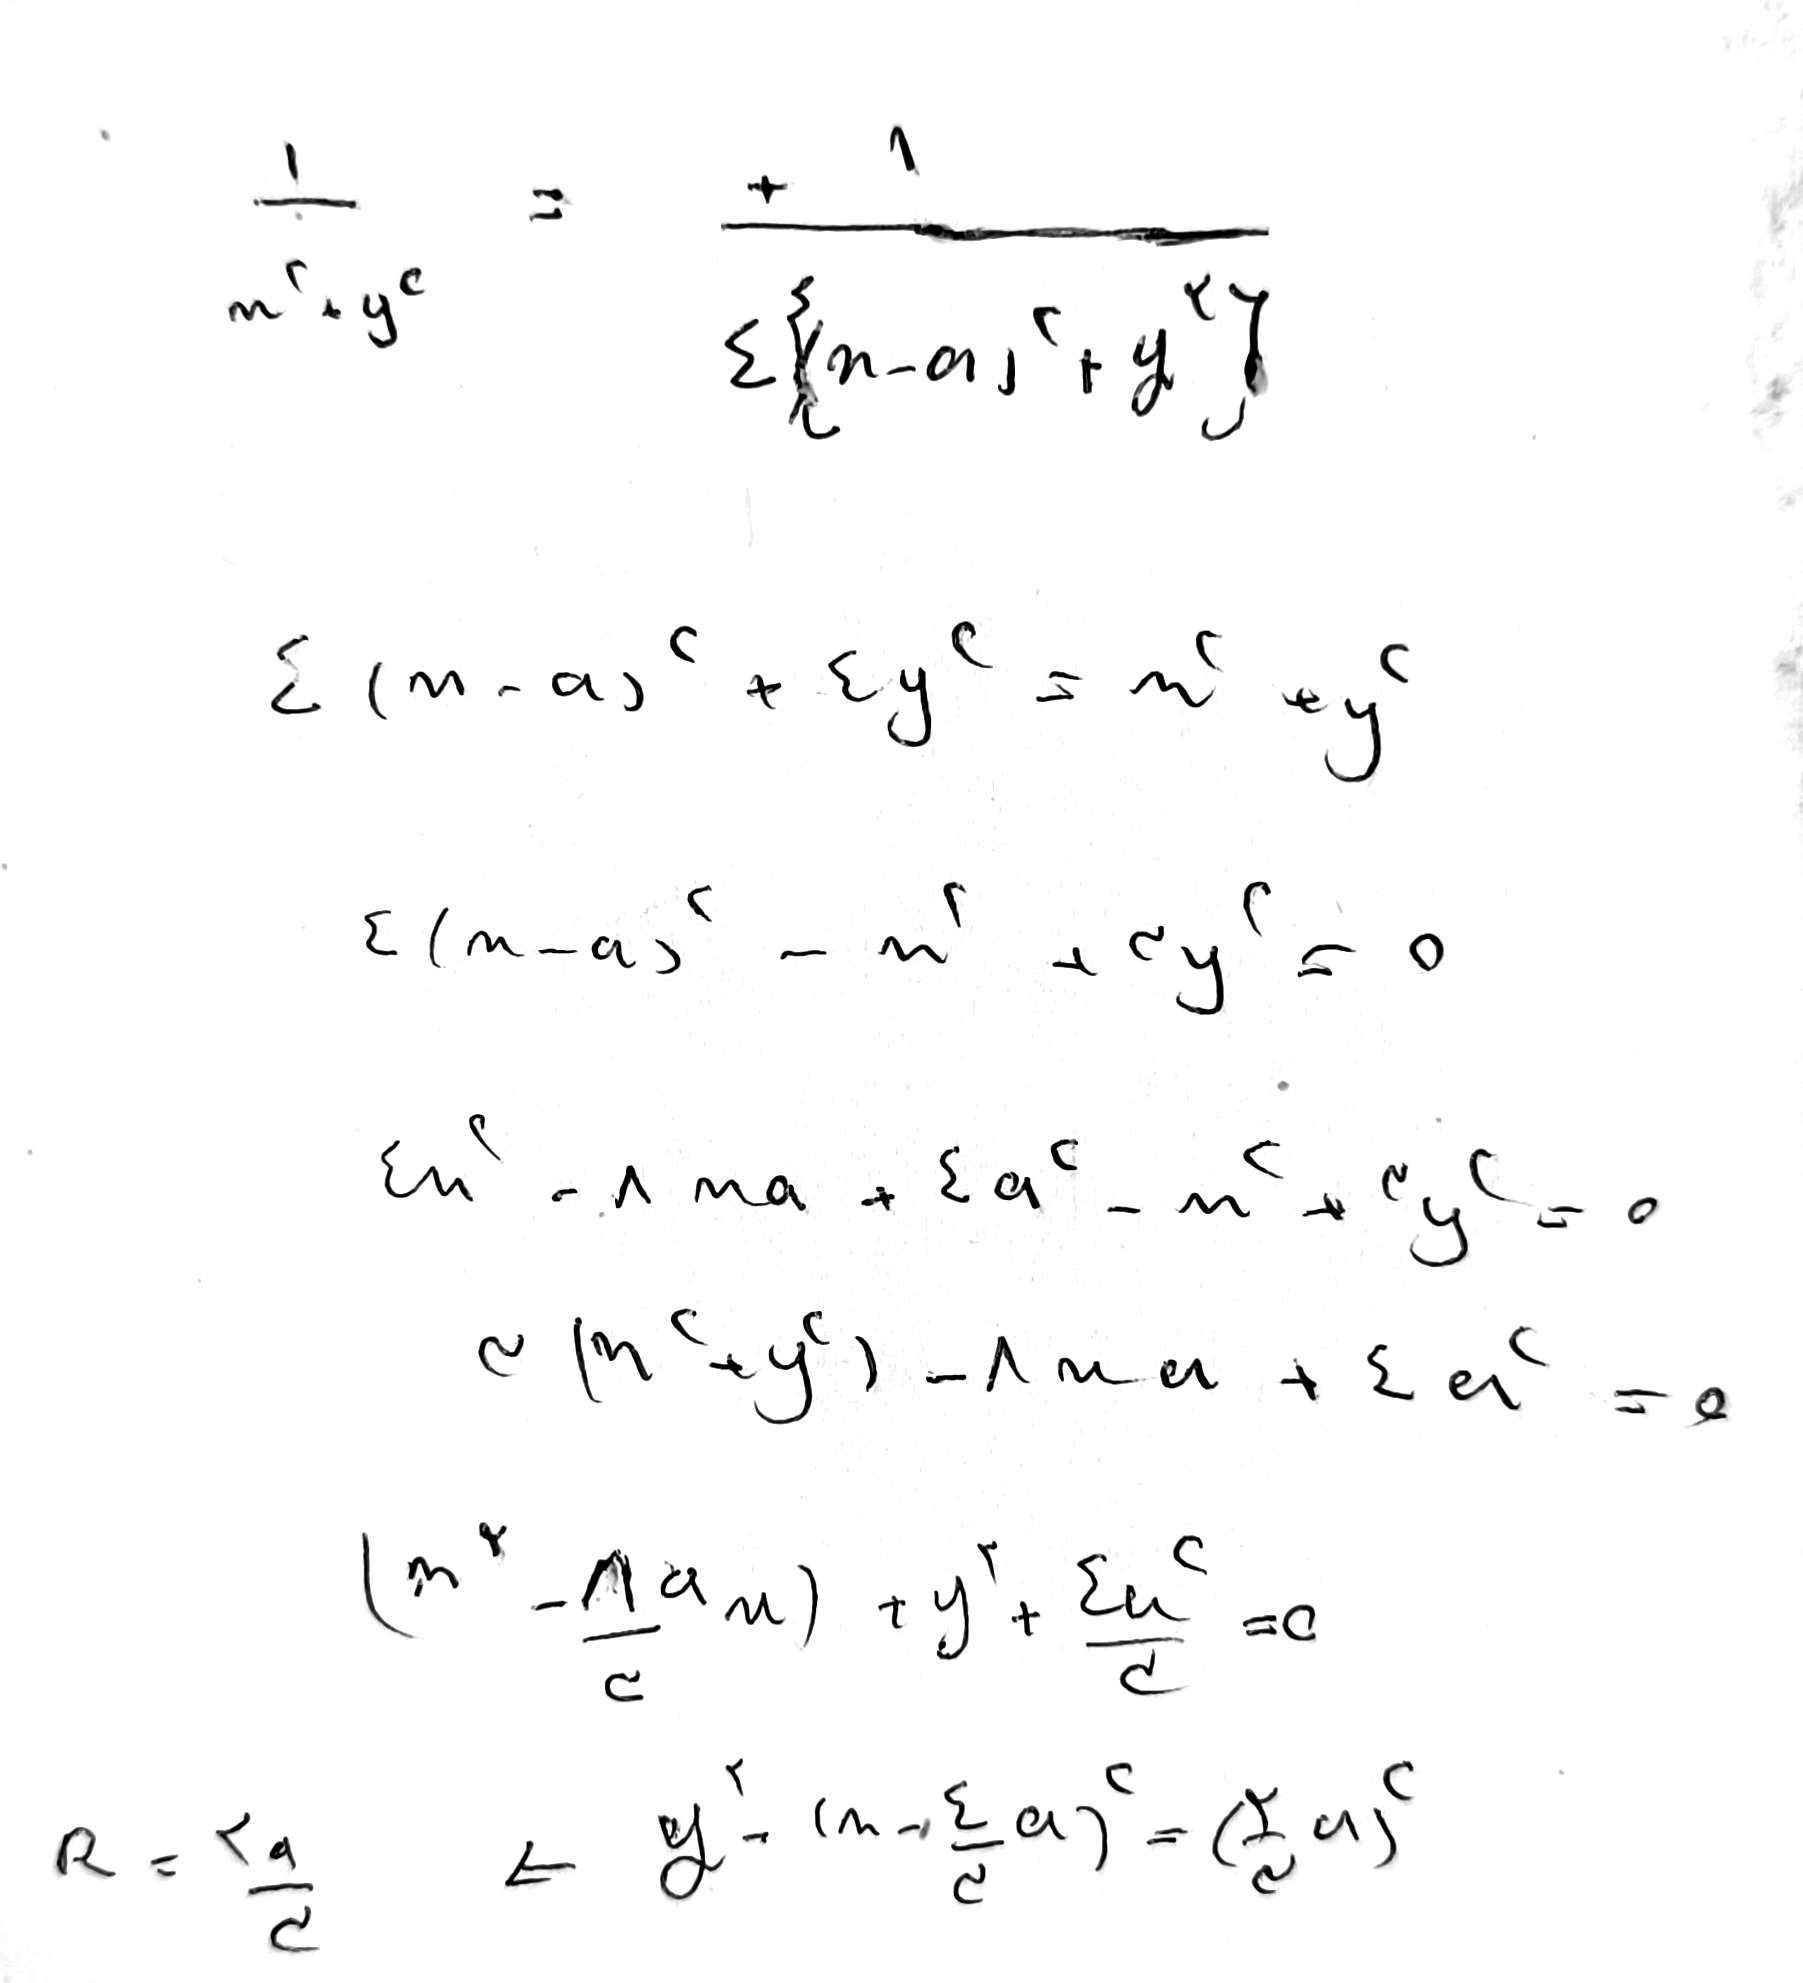
\includegraphics[width=0.7\textwidth]{2.8-so}
\end{figure}
اگر $a=1$ باشد که طبق آن در نمودار پتانسیل سوال قبل درنظر گرفتم داریم:
\[ R = 2/3 = 0.66 \]

\newpage
\subsection{}
از مسئله ۲.۵ میدانیم که پتانسیل قرص بردار است:
\[ \varphi = \frac{\sigma}{2\epsilon_0}[ \sqrt{R^2 + Z^2}+|Z|] \]
پس داریم:
\begin{figure}[h!]
\centering
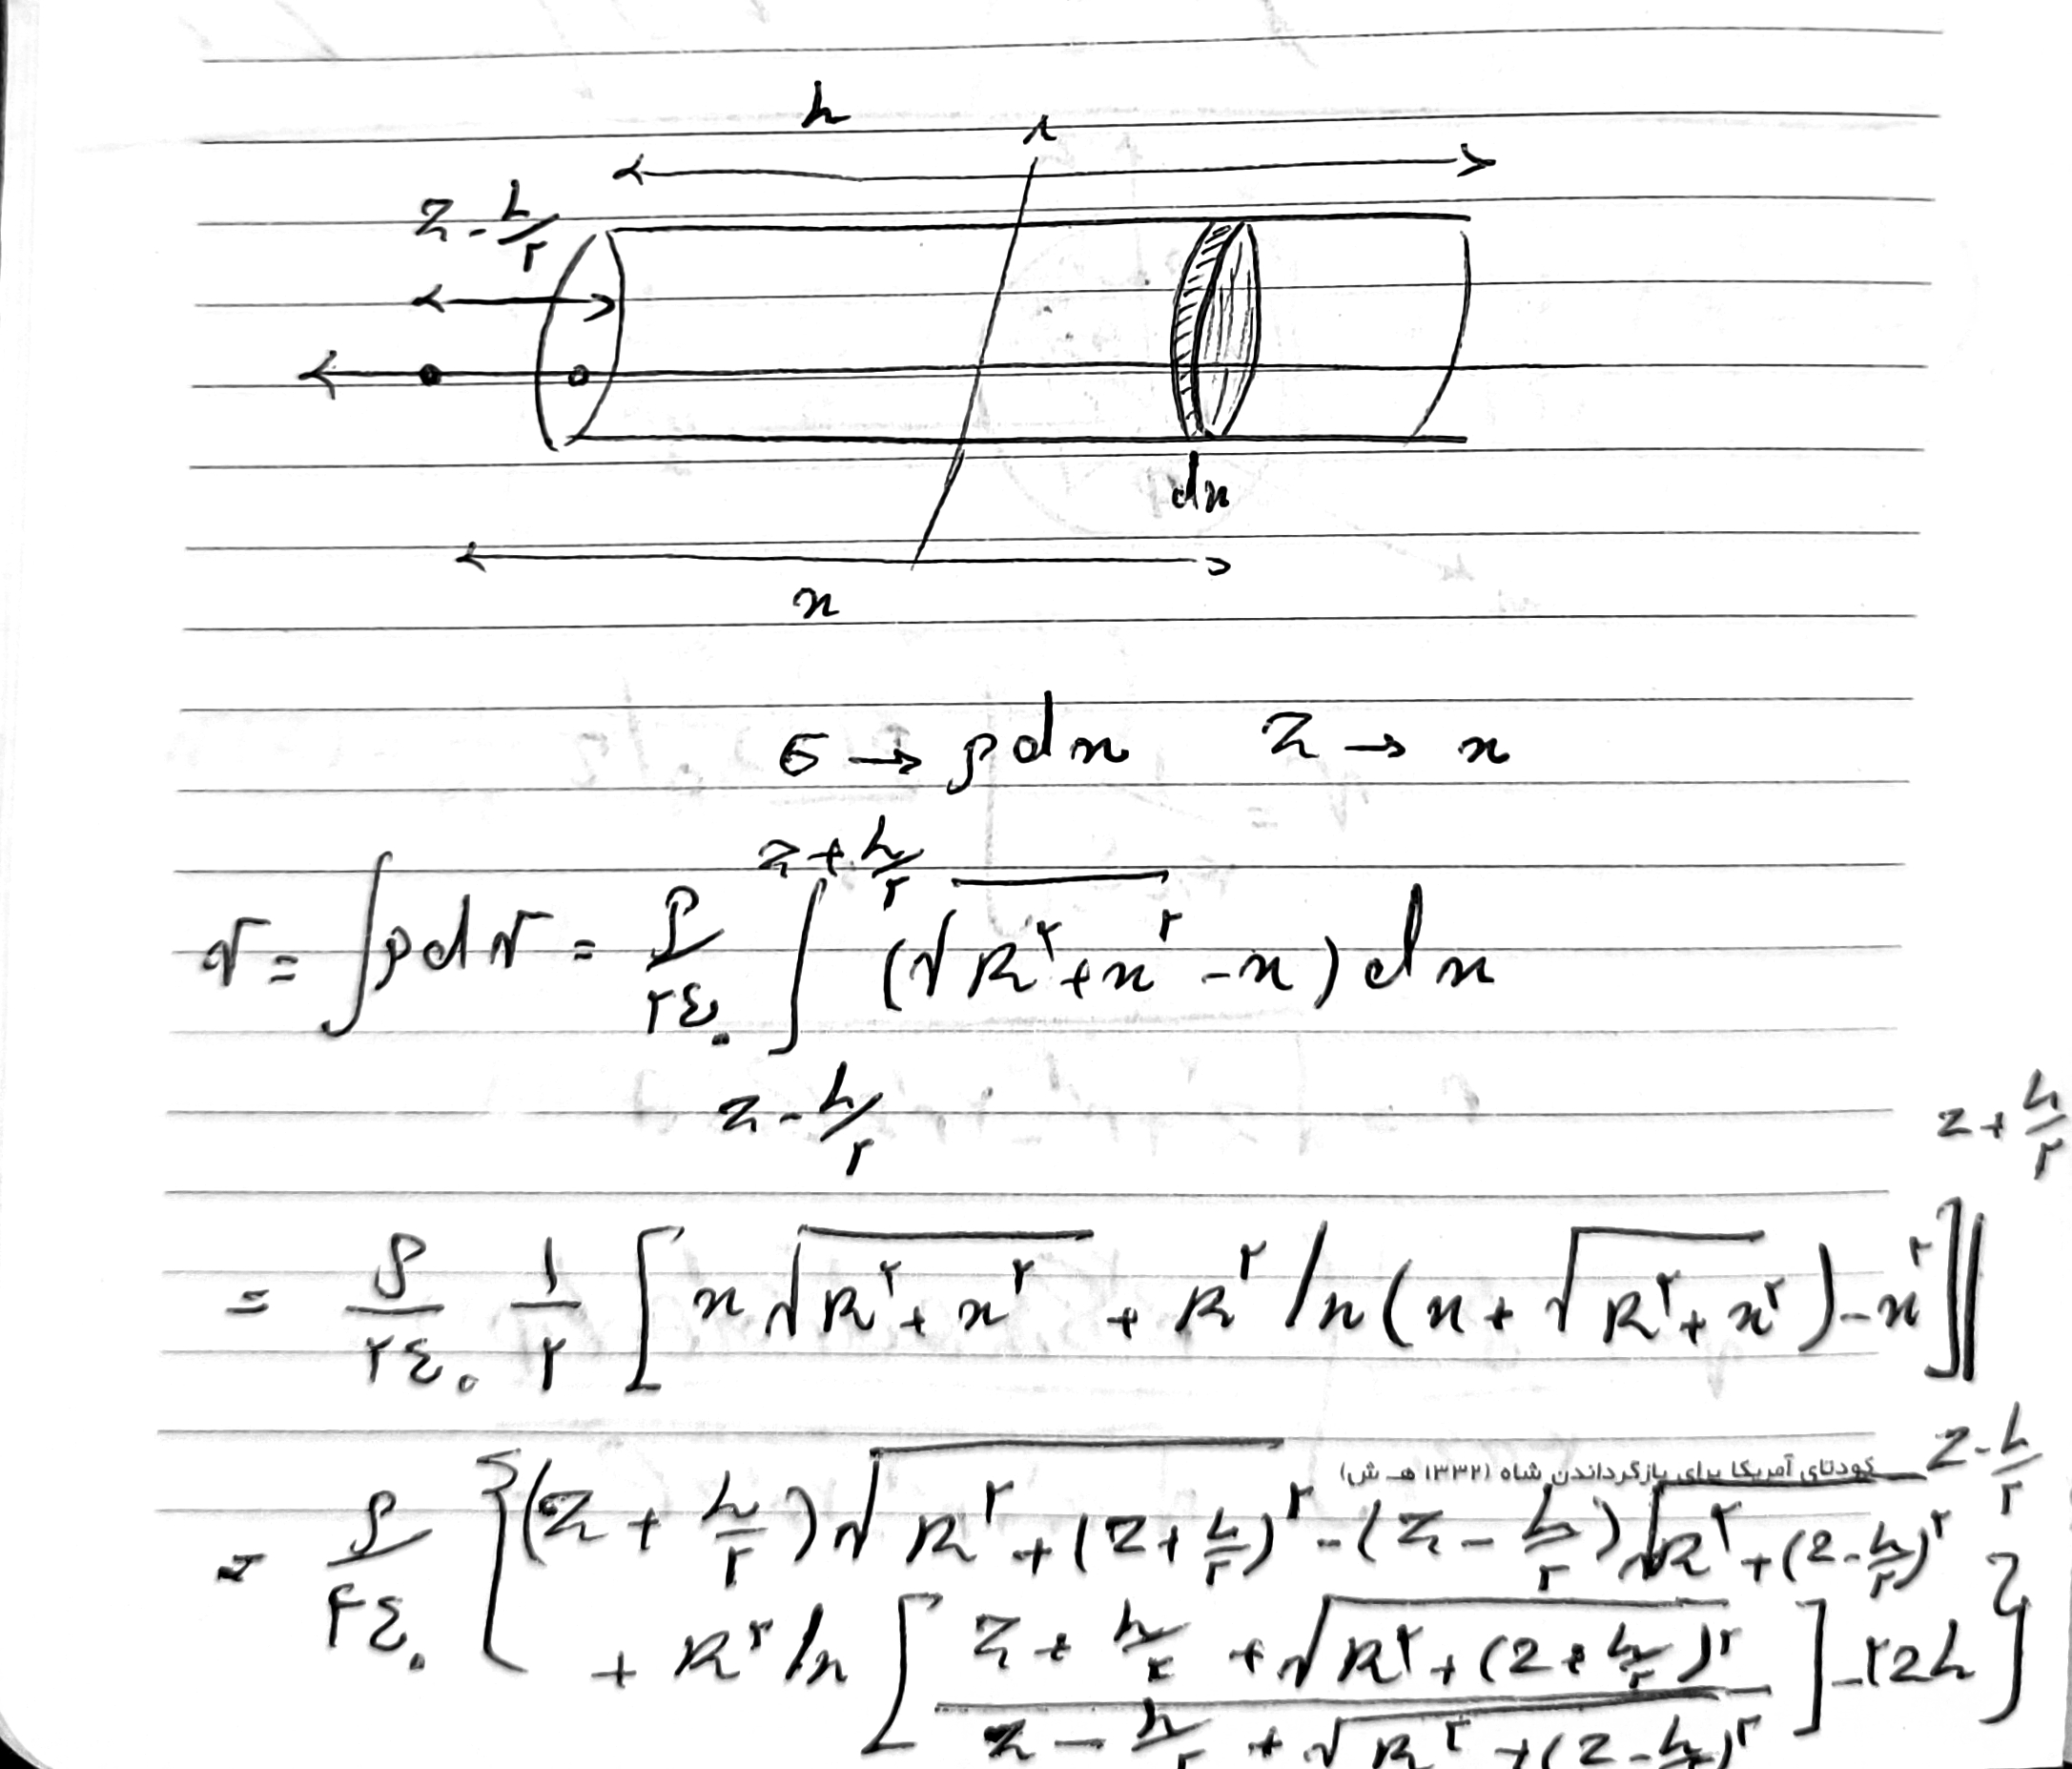
\includegraphics[width=0.9\textwidth]{2.9-so}
\end{figure}
\newpage
\subsection{}
\begin{figure}[h!]
\centering
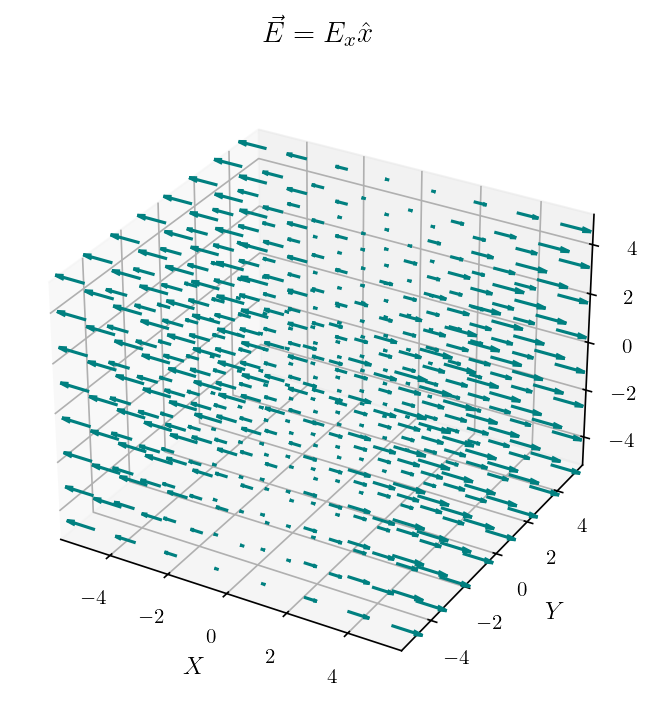
\includegraphics[width=0.5\textwidth]{2.10plt}
\end{figure}
\[ \varphi =  \oint_C \vec{E}\cdot d\vec{r}= \int_{x}^{x+\Delta x} E_x dx - \int_{x+ \Delta x}^{x} {E_x}' dx = (E_x - {E_x}')\Delta x \neq 0\]
یا
\[ \vec{\nabla} \times \vec{E} = 0 \]
\[
\begin{vmatrix} 
\hat{x} & \hat{y} & \hat{z} \\ 
\partial_x & \partial_y & \partial_z \\ 
E_x & 0 & 0 
\end{vmatrix} = 0\hat{x} + 0\hat{y} + 0\hat{z} \]

\subsection{}
الف)

\[ x^2 + y^2 + z^2 = R^2 \]
\[ \Vert \vec{E}\Vert = \frac{1}{4\pi \epsilon_0} \frac{q}{R^2} \]
\[ \varphi = -\int_{\infty}^{R} \vec{E} \cdot d\vec{r} = \frac{1}{4\pi \epsilon_0} \frac{q}{R} \]
\[ \varphi = 3 \times 10^6 \times 0.08 = 24 \times 10^4 V \]

ب)

\[ R = \sqrt{\frac{q}{r\pi \epsilon_0 E}} = 54.8 \\ m \]

\subsection{}
\begin{figure}[h!]
\centering
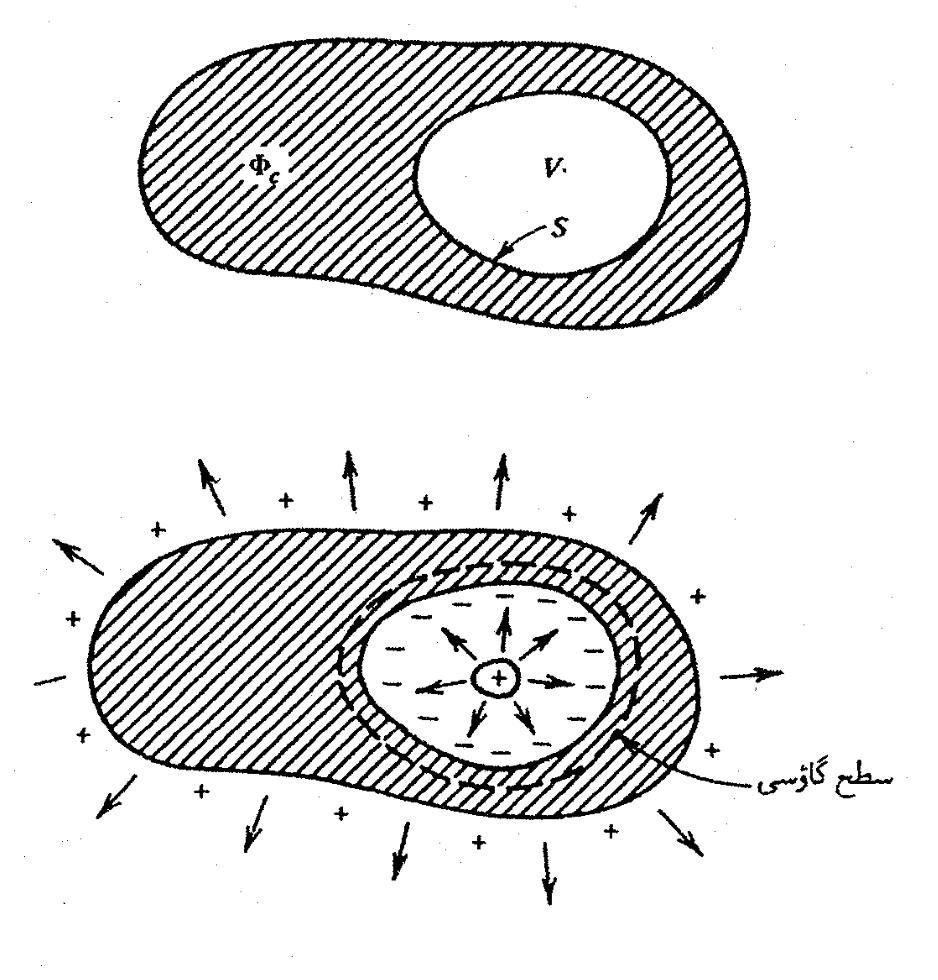
\includegraphics[width=0.5\textwidth]{2.12fig}
\end{figure}
اگر از قانون گاوس برای یک سطح بسته در داخل رسانا استفاده کنیم، می‌دانیم که چون در داخل رسانا $\vec{E}=0$، در این صورت
\[ \oint_{S} \vec{E}(\vec{r})\cdot d\vec{a}=0 \]
و در نتیجه $Q_{int}=0$، از این رو نتیجه می‌گیریم که بر روی سطح داخلی رسانا یک بار مخالف ($-q$) القا می‌شود که باعث صفر‌شدن میدان جسم باردار می‌شود.
\newpage
\subsection{}
الف)
\begin{figure}[h!]
\centering
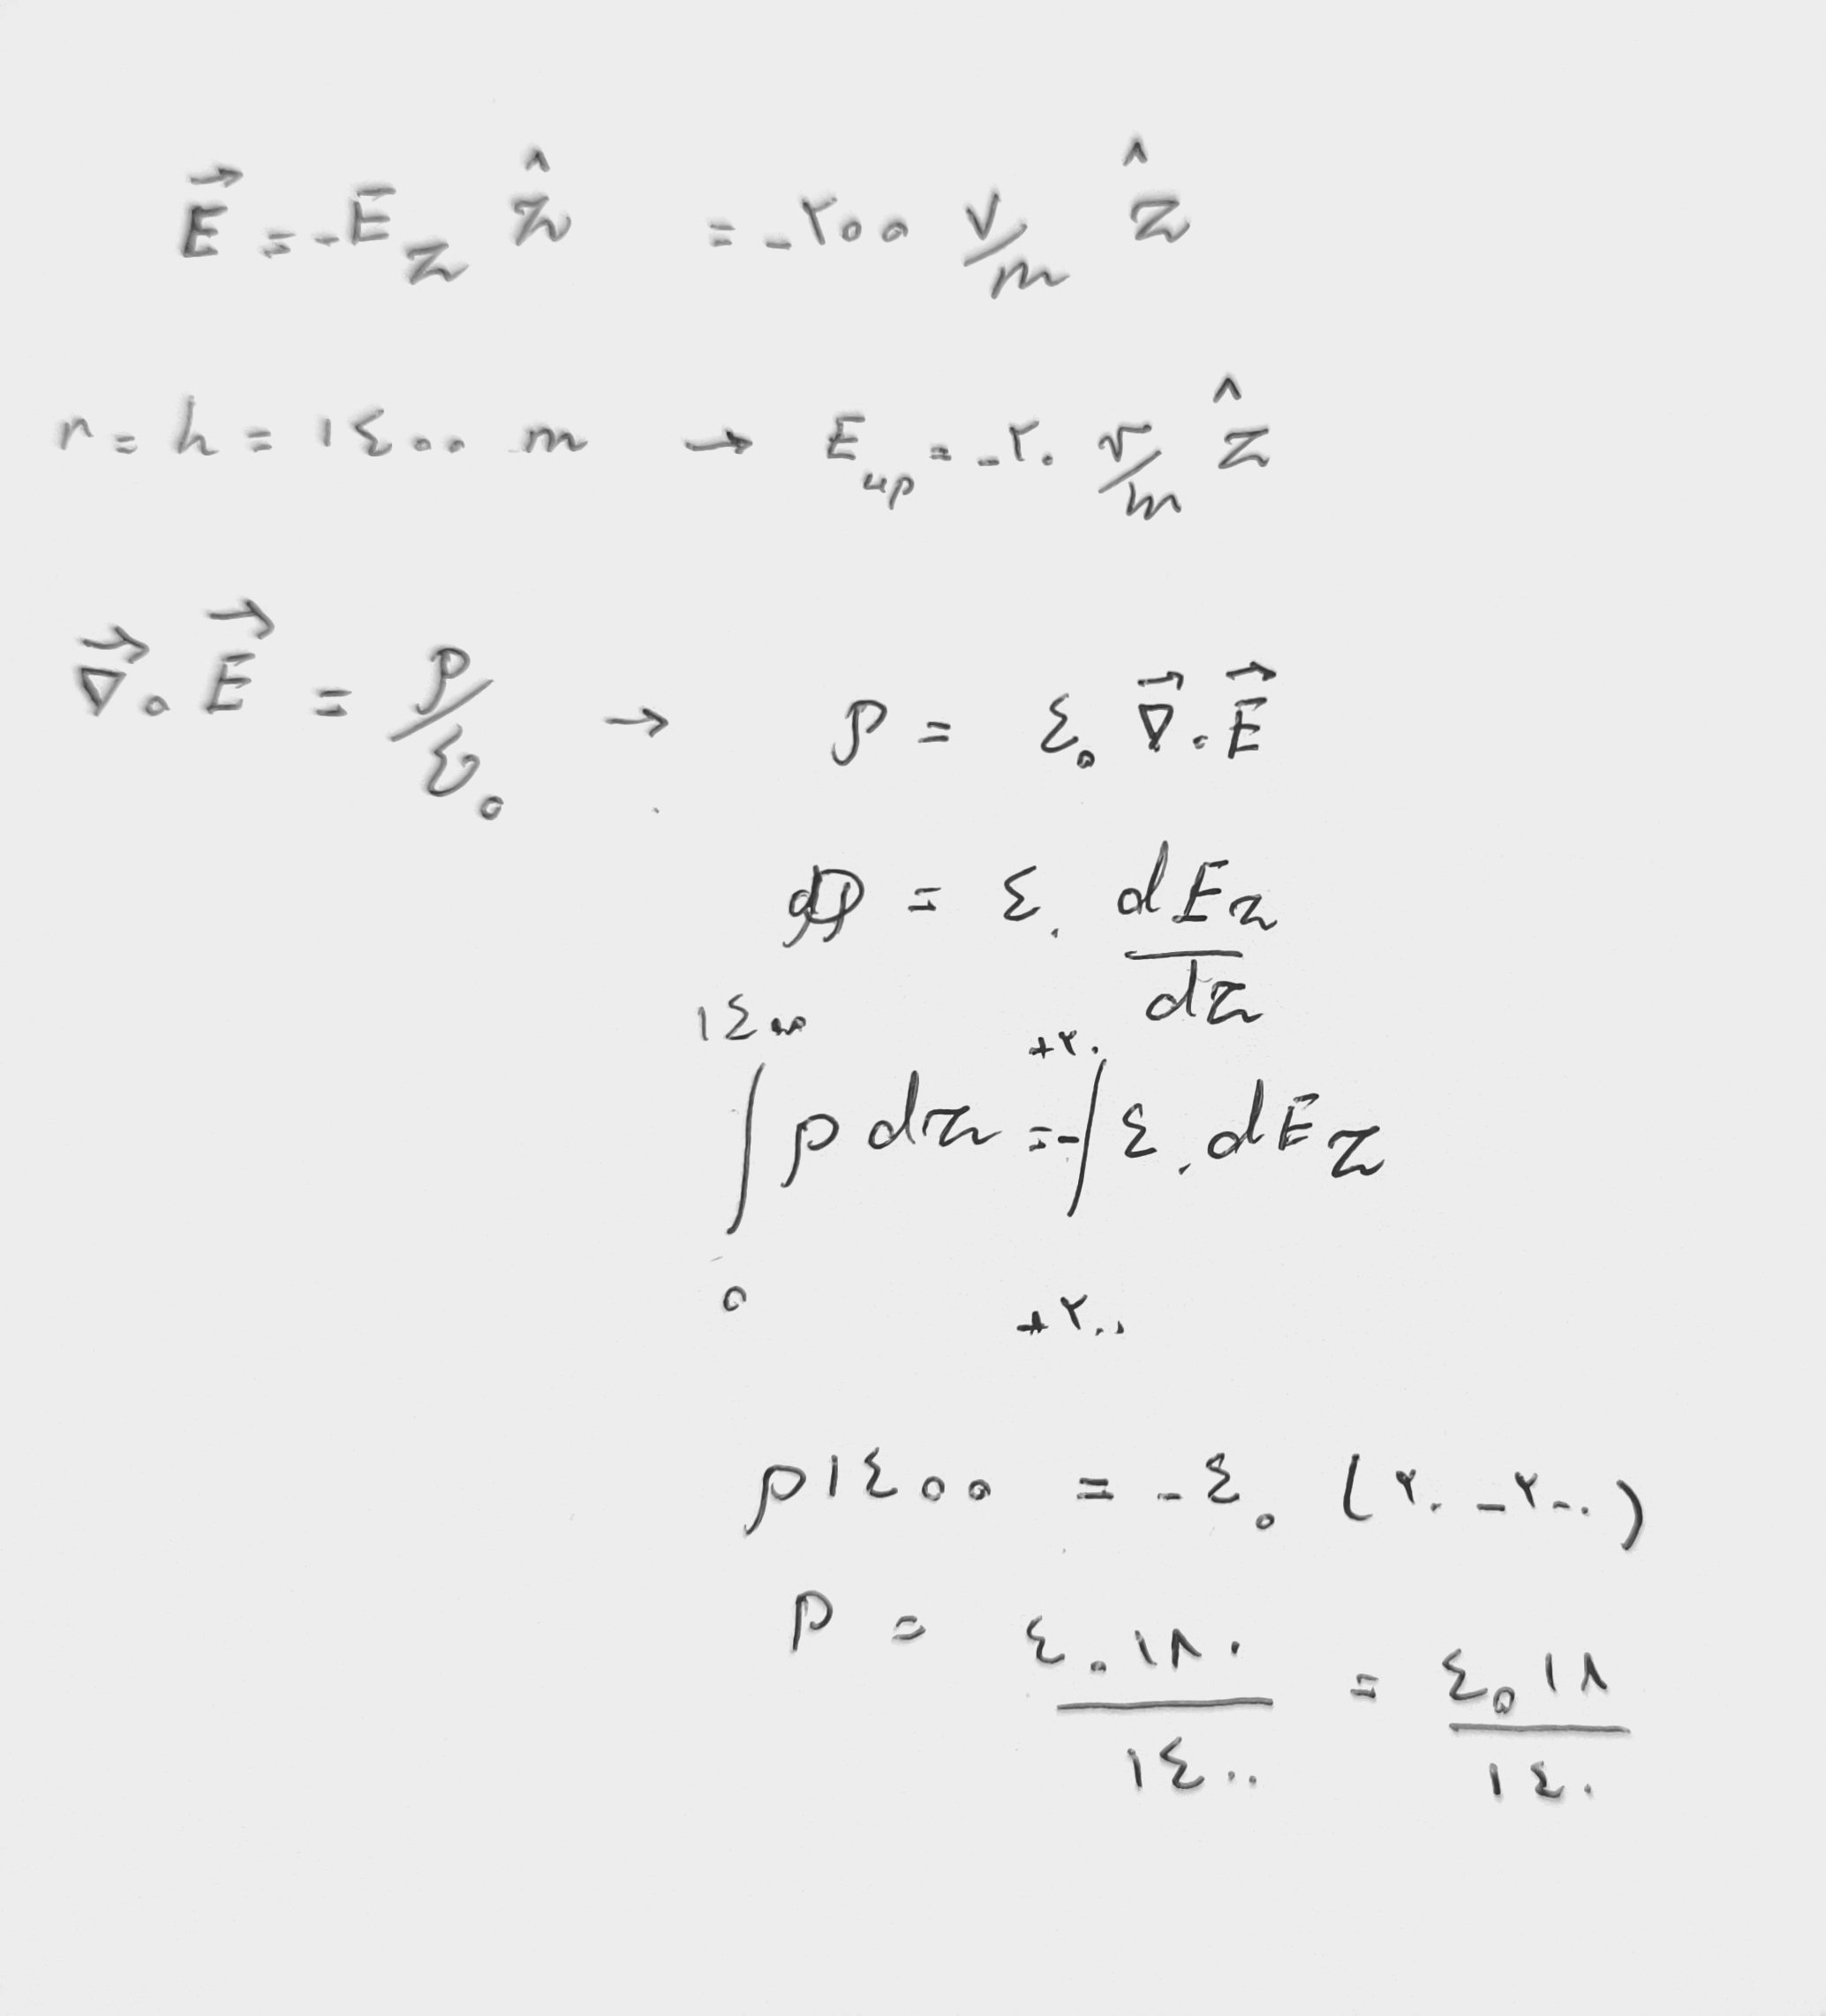
\includegraphics[width=0.5\textwidth]{2.13-so}
\end{figure}

ب) مثبت

\subsection{}

\begin{figure}[h!]
\centering
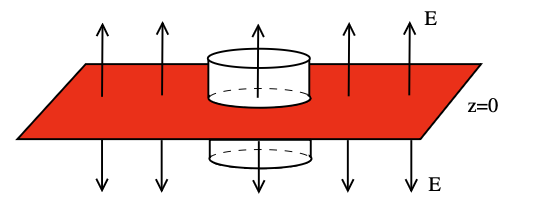
\includegraphics[width=0.6\textwidth]{2.14fig}
\end{figure}

فرض کنید دو صفحه نامتناهی و موازی در صفحات $z = 0$ و $z = d$ قرار دارند. صفحه اول در $z = 0$ دارای چگالی سطحی بار $\sigma > 0$ و صفحه دوم در $z = d$ دارای چگالی سطحی بار $-\sigma$ است. 

طبق توضیحات زیر، میدان الکتریکی حاصل از یک صفحه نامتناهی با چگالی سطحی بار یکنواخت به صورت زیر است که همواره به سمت خارج از صفحه (برای بار مثبت) یا به سمت داخل صفحه (برای بار منفی) جهت‌گیری می‌کند و بزرگی آن مستقل از فاصله است:

\[ \int_S \vec{E} \cdot d\vec{S} = E(z)A-E(-z)A=2E(z)A=\frac{\sigma A}{\epsilon_0} \quad \longrightarrow E(z) = \frac{\sigma}{2\epsilon_0} \]

\begin{figure}[h!]
\centering
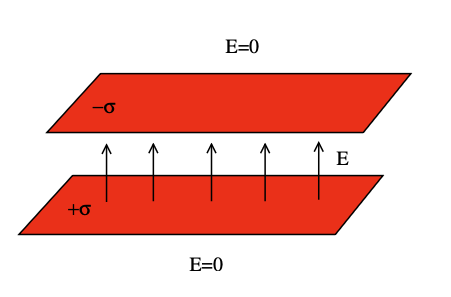
\includegraphics[width=0.6\textwidth]{2.14fig2}
\end{figure}

الف) ($0 < z < d$):

\[ \vec{E}_{+} = \frac{\sigma}{2\epsilon_0} \hat{z} ,\quad \vec{E}_{-} = \frac{\sigma}{2\epsilon_0} \hat{z} \]

\[ \vec{E}_{\text{total}} = \vec{E}_{+} + \vec{E}_{-} = \frac{\sigma}{2\epsilon_0} \hat{z} + \frac{\sigma}{2\epsilon_0} \hat{z}= \frac{\sigma}{\epsilon_0} \hat{z} \]

ب)

($z > d$):

\[ \vec{E}_{+} = \frac{\sigma}{2\epsilon_0} \hat{z} , \quad \vec{E}_{-} = -\frac{\sigma}{2\epsilon_0} \hat{z} \]

\[ \vec{E}_{\text{tot}} = \frac{\sigma}{2\epsilon_0} \hat{z} + \left( -\frac{\sigma}{2\epsilon_0} \hat{z} \right) = \vec{0} \]

($z < 0$):
\[ \vec{E}_{+} = -\frac{\sigma}{2\epsilon_0} \hat{z} , \quad \vec{E}_{-} = \frac{\sigma}{2\epsilon_0} \hat{z} \]
\[ \vec{E}_{\text{total}} = -\frac{\sigma}{2\epsilon_0} \hat{z} + \frac{\sigma}{2\epsilon_0} \hat{z} = \vec{0} \]

\newpage
\subsection{}
الف)

\begin{figure}[h!]
\centering
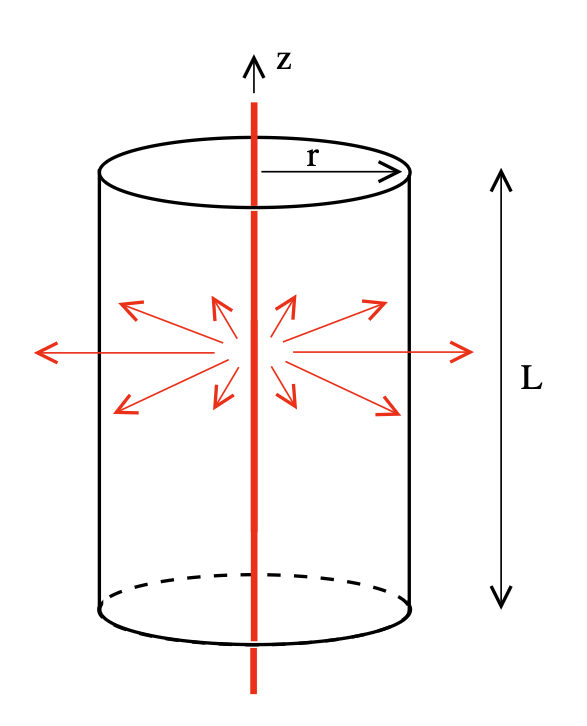
\includegraphics[width=0.2\textwidth]{2.15fig}
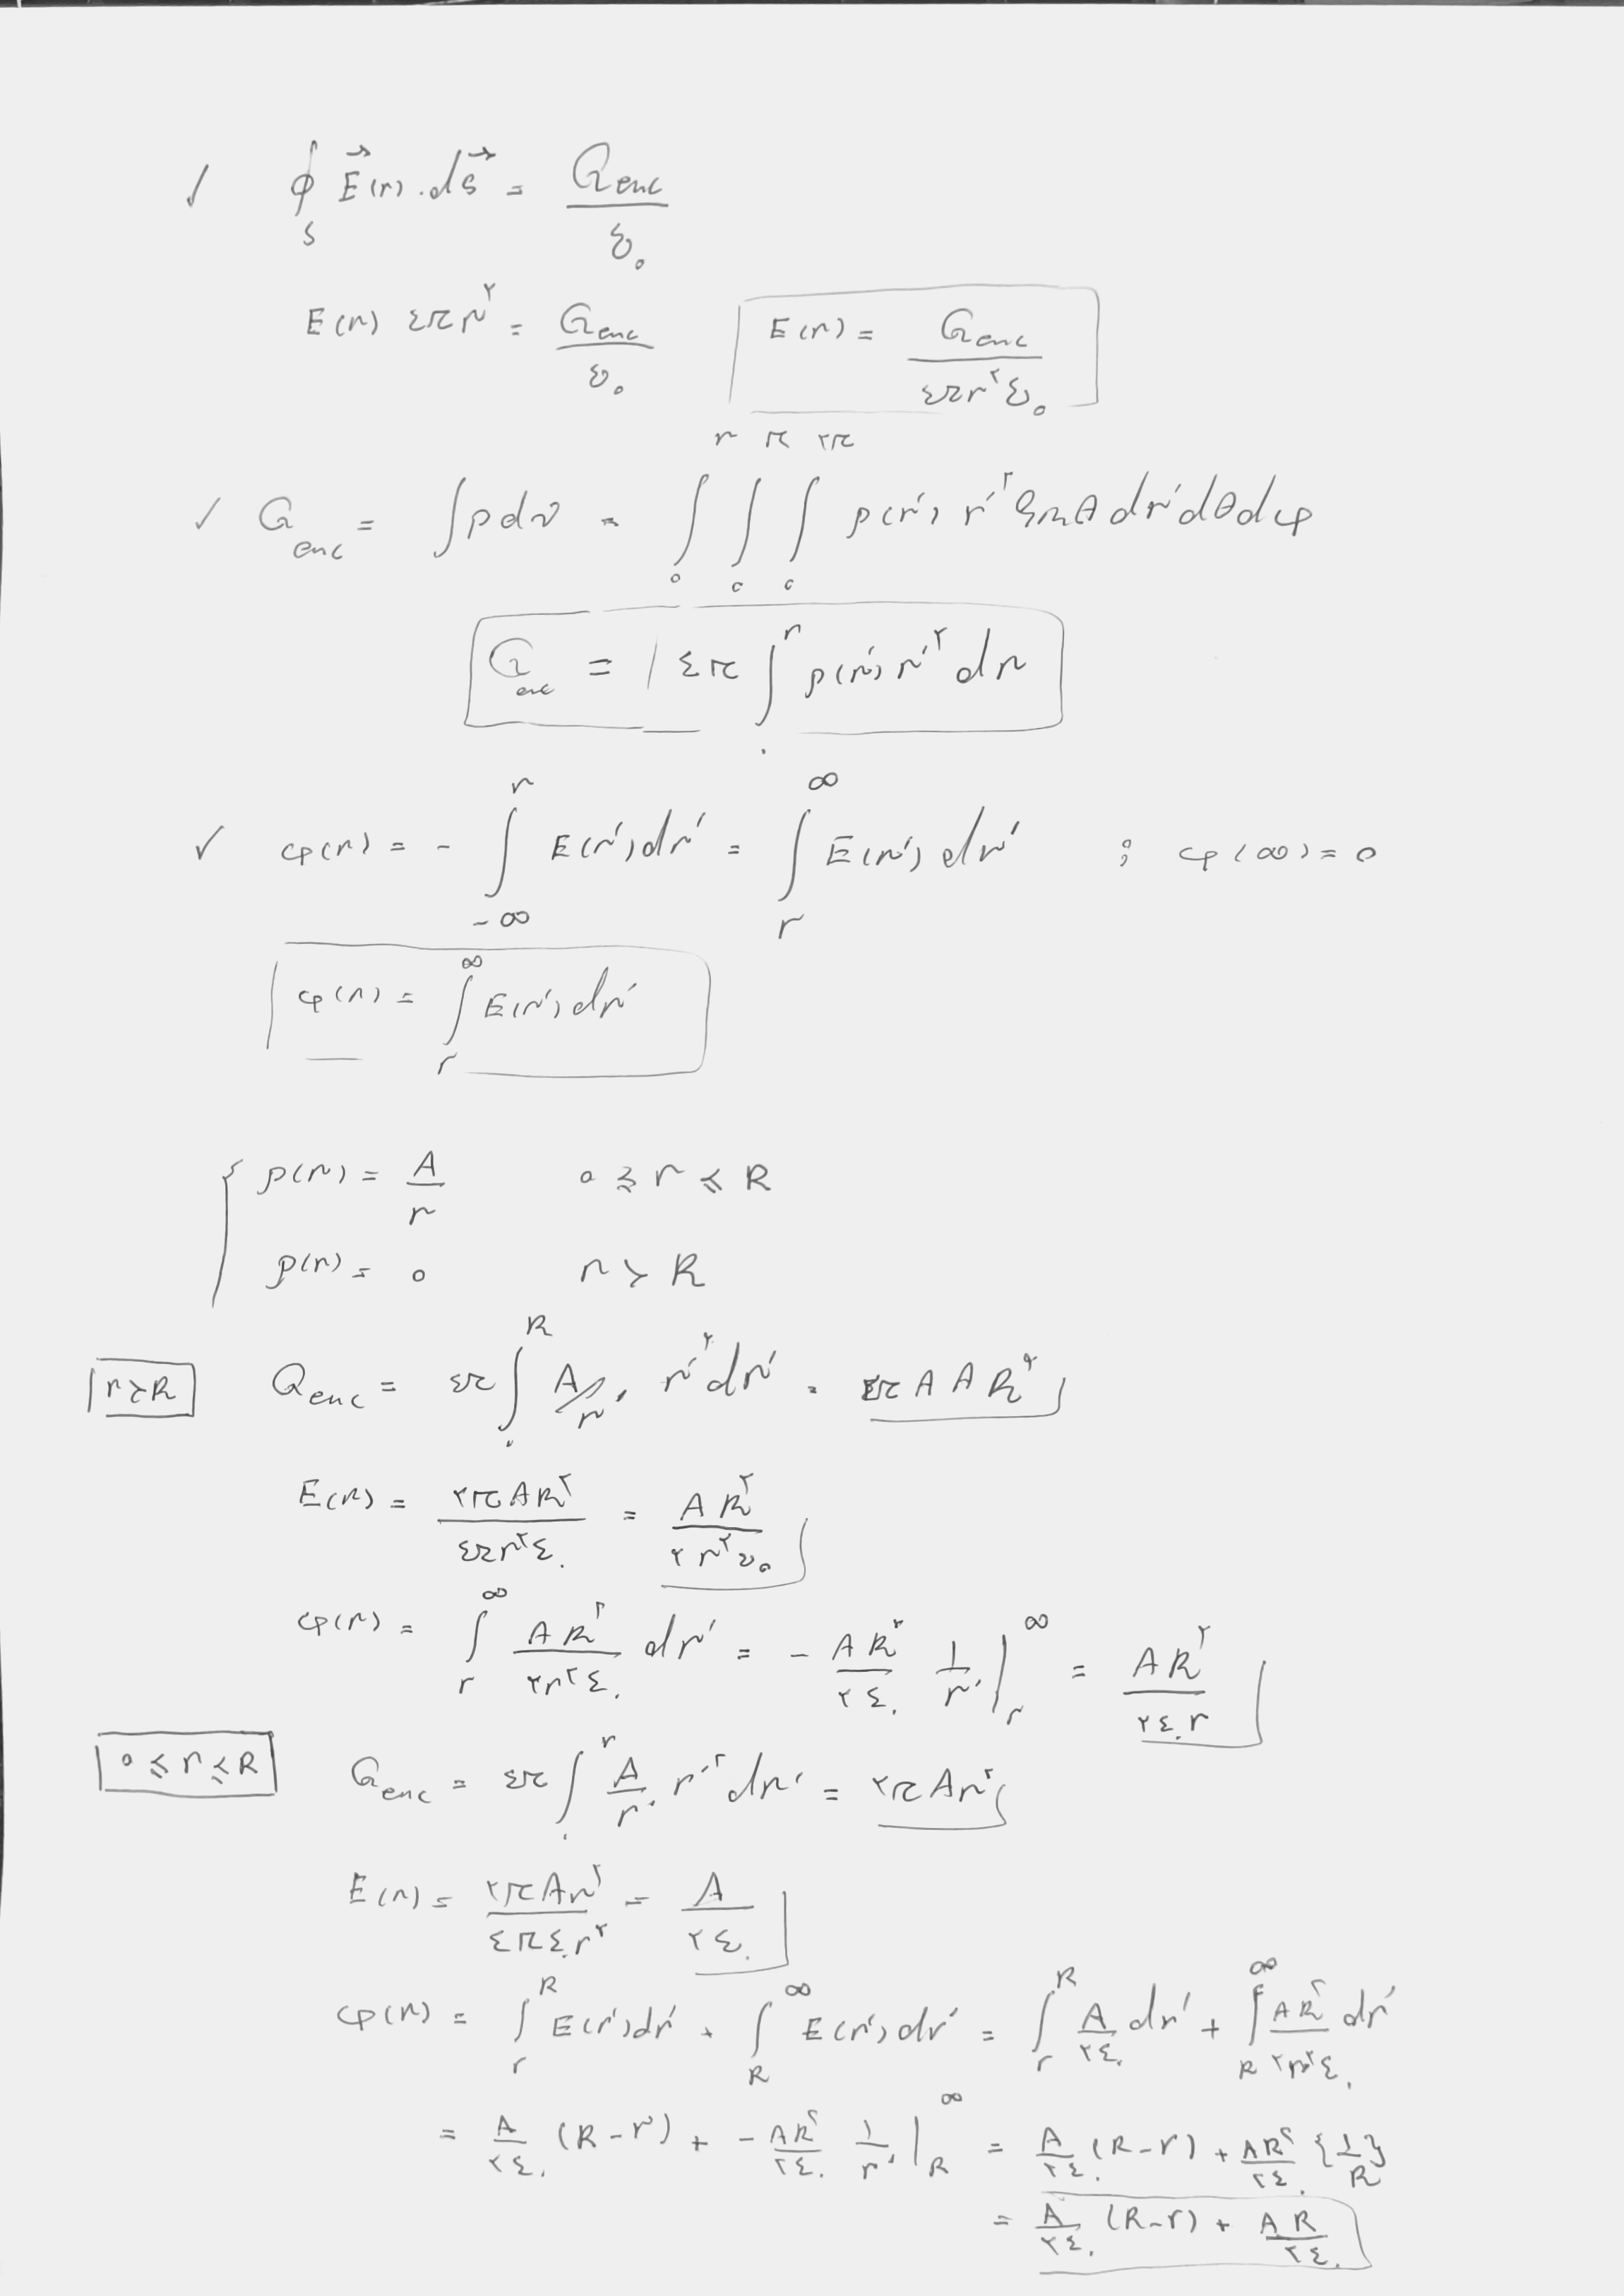
\includegraphics[width=0.5\textwidth]{2.15-so1}
\end{figure}

ب)

\begin{figure}[h!]
\centering
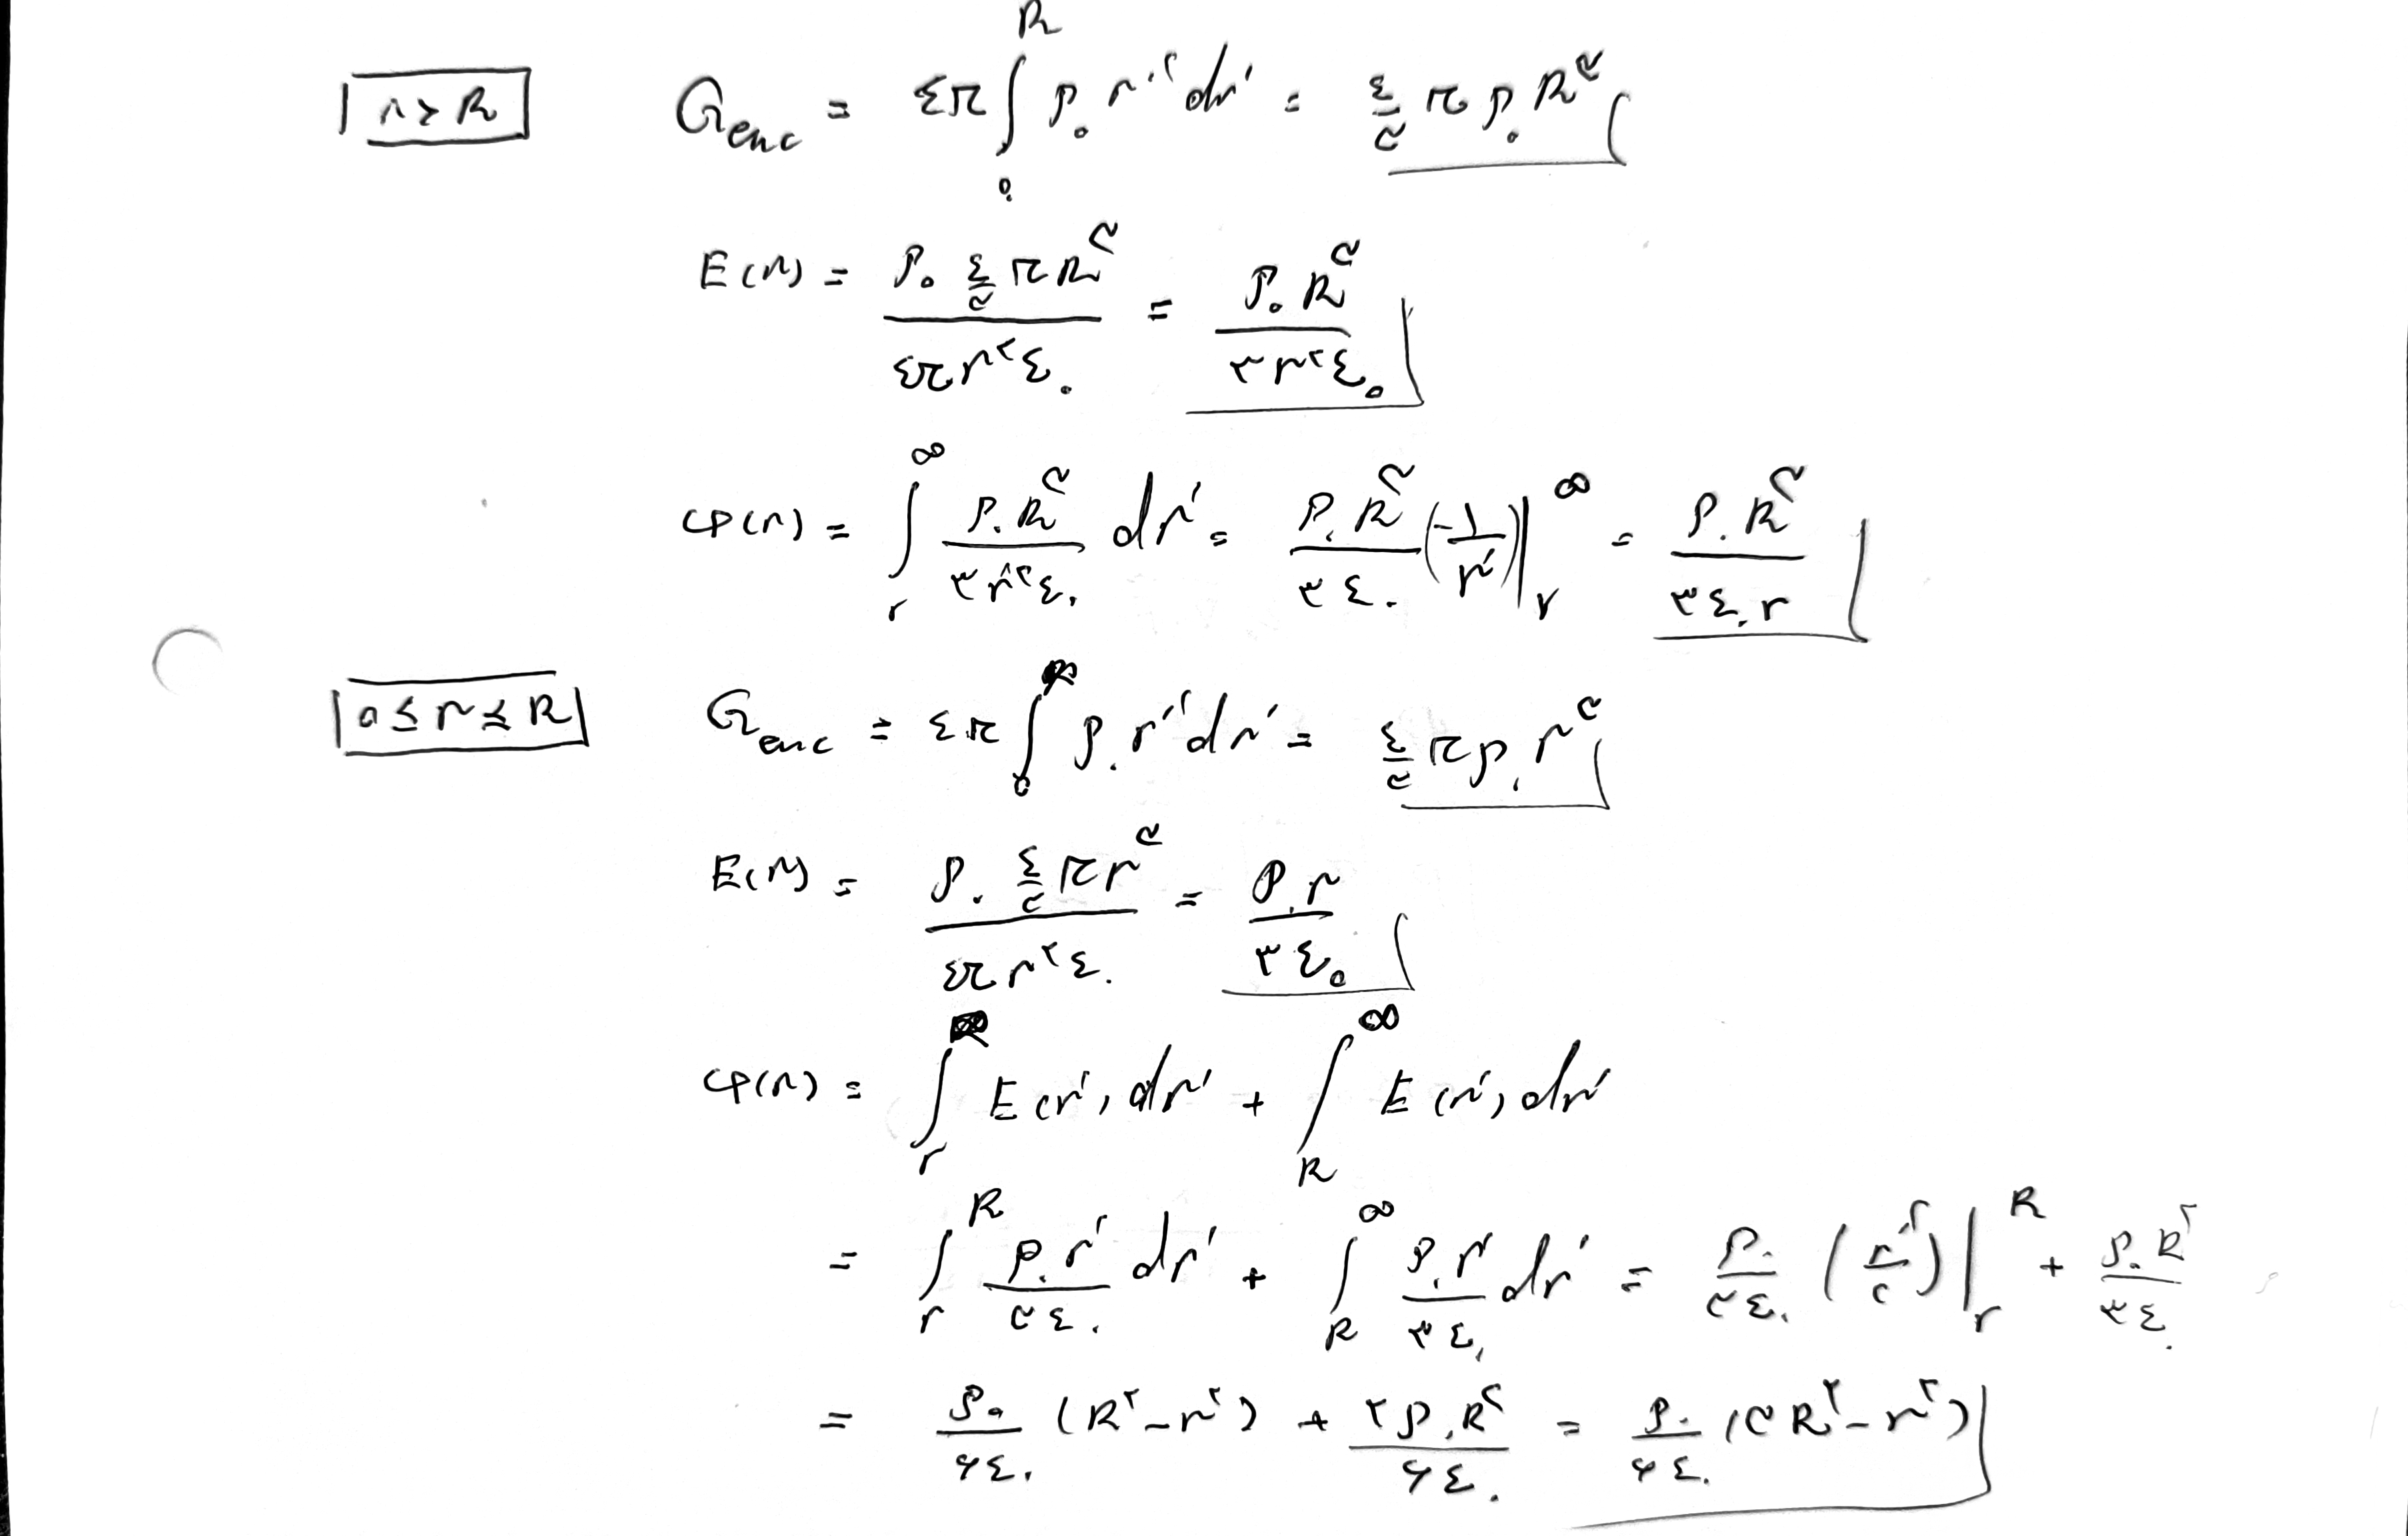
\includegraphics[width=0.55\textwidth]{2.15-so2}
\end{figure}

\subsection{}

$(r>R)$:

\[ Q_{enc} = \int \rho d\nu = \int_{0}^{R} \int_{0}^{2\pi} \int_{-l/2}^{l/2} \rho r dr d\theta dz = \rho R^2 \pi l\]

\[ \oint_S \vec{E}.d\vec{s} = \frac{Q_{enc}}{\epsilon_0} \]
\[ E_r = \frac{\rho \pi R^2 l}{\epsilon_0 2\pi rl} \]
\[ E_r = \frac{\rho R^2}{2\epsilon_0 r} \]

$(r<R)$:

\[ Q_{enc} = \int \rho d\nu = \int_{0}^{r} \int_{0}^{2\pi} \int_{-l/2}^{l/2} \rho r dr d\theta dz = \rho r^2 \pi l\]

\[ \oint_S \vec{E}.d\vec{s} = \frac{Q_{enc}}{\epsilon_0} \]
\[ E_r = \frac{\rho \pi r^2 l}{\epsilon_0 2\pi rl} \]
\[ E_r = \frac{\rho r}{2\epsilon_0} \]

\subsection{}

\newpage
\section{فصل سوم: حل‌المسائل الکترواستاتیک}

\section{فصل چهارم: میدان الکترواستاتیک در محیط‌های دی‌الکتریک}

\end{document}